\documentclass[lettersize,journal]{IEEEtran}
\usepackage{amsmath,amsfonts}
\usepackage{algorithmic}
\usepackage{orcidlink}
\usepackage{booktabs}
\usepackage{algorithm}
\usepackage{xcolor}
\usepackage{multirow}
\usepackage{array}
\usepackage[caption=false,font=normalsize,labelfont=sf,textfont=sf]{subfig}
\usepackage{textcomp}
\usepackage{stfloats}
\usepackage{url}
\usepackage{verbatim}
\usepackage{graphicx}
\usepackage{gensymb}
\usepackage{cite}
\renewcommand{\textcolor}[2]{#2}
\hyphenation{op-tical net-works semi-conduc-tor IEEE-Xplore}
% updated with editorial comments 8/9/2021

\begin{document}

\title{UTDT: A Baseline Benchmark for Urban Traffic \\ Flow Digital Twins via Roadside \\ LiDAR-Camera Fusion}

\author{\hypersetup{
		colorlinks=false,
		pdfborder={0 0 0}
	}Haidong~Wang\raisebox{0.8ex}{\orcidlink{0000-0002-4614-5817}},~Pengfei~Xiao\raisebox{0.8ex}{\orcidlink{0009-0003-6278-463X}},Ao~Liu\raisebox{0.8ex}{\orcidlink{0009-0006-9153-4295}}, Jianhua~Zhang\raisebox{0.8ex}{\orcidlink{0009-0009-9097-8523}},~and Qia~Shan\raisebox{0.8ex}{\orcidlink{0009-0004-0279-7807}}
        % <-this % stops a space

\thanks{Haidong Wang is with Hunan University of Technology and Business, Changsha 410082, China, and Xiangjiang Laboratory; Pengfei Xiao, Ao Liu, Jianhua Zhang and Qia Shan are with Hunan University Of Technology and Business, Changsha 410082, China (e-mail: whd@hutb.edu.cn; 2893666867@qq.com; 2496556459@qq.com; zhangjianhua6682@126.com; s540534349@163.com).(\textit{Corresponding author: Haidong Wang.})
}}
%\thanks{H. Wang is with Hunan University of Technology and Business, Changsha 410082, China, and %Xiangjiang Laboratory; P. Xiao, A. Liu, J. Zhang and Q. Shan are with Hunan University Of Technology %and Business, Changsha 410082, China (e-mail: whd@hutb.edu.cn; 2893666867@qq.com; 2496556459@qq.com; %zhangjianhua6682@126.com; s540534349@163.com).
	
% <-this % stops a space
 %\thanks{Manuscript received April 19, 2021; revised August 16, 2021.}}

% The paper headers
\markboth{Journal of \LaTeX\ Class Files,~Vol.~14, No.~8, August~2021}%
{Shell \MakeLowercase{\textit{et al.}}: A Sample Article Using IEEEtran.cls for IEEE Journals}

%\IEEEpubid{0000--0000/00\$00.00~\copyright~2021 IEEE}
% Remember, if you use this you must call \IEEEpubidadjcol in the second
% column for its text to clear the IEEEpubid mark.

\maketitle

\begin{abstract}
Digital twin (DT) technology has emerged as a key enabler for bridging the gap between physical and virtual worlds, providing real-time synchronization, monitoring, and optimization capabilities.
However, in the field of intelligent transportation and autonomous driving, most existing DT systems remain limited to single-scene simulations or simplified traffic models, lacking the ability to maintain spatiotemporal consistency and continuous vehicle identities across multiple intersections.
To address these limitations, this paper proposes an Urban Traffic Flow Digital Twin (UTDT) framework that builds a high-fidelity, multi-scene representation of traffic flow.
UTDT integrates four core modules: single-intersection multi-object tracking, multi-intersection trajectory association, trajectory inference and restoration, and twinning synchronization.
Multi-object tracking is enhanced by fusing LiDAR and camera data and leveraging re-identification for cross-scene identity continuity, enabling accurate trajectory reconstruction and precise digital twin–based vehicle control in complex traffic scenarios.
The experimental results show that UTDT can provide high-fidelity simulation scenarios for the testing and optimization of autonomous driving systems, which promotes the development of intelligent transportation systems and provides important support for the construction of future smart cities.
\begingroup
\hypersetup{pdfborder={0 0 0}}The source code and datasets are available at \url
{https://github.com/OpenHUTB/traffic\_twin}.
\endgroup
\end{abstract}

\begin{IEEEkeywords}
digital twins, autonomous driving, vehicle detection, multi-object tracking, trajectory restoration.
\end{IEEEkeywords}

\section{Introduction}
\IEEEPARstart{W}{ith} the rapid development of intelligent transportation, autonomous driving, and urban management, digital twin technology, as an important innovative tool, has gradually shown tremendous potential in various fields\cite{Alpher17}. 
A digital twin refers to the creation of a digital model corresponding to the real world through the real-time synchronization of data collected from the physical world and virtual models\cite{Alpher20c}. 
This technology can simulate, analyze, and optimize the real world in a virtual environment, thus providing support for decision-making\cite{Alpher21b}. 
In the field of autonomous driving, digital twin technology can accurately replicate factors such as traffic flow, road structure, and pedestrian behavior, providing a precise testing and training environment for the perception, planning, and control of autonomous driving systems\cite{Alpher24}\cite{Alpher20d}.

However, existing digital twin research often focuses on static modeling or the reproduction of local traffic scenarios, lacking accurate characterization of dynamic traffic flows and cross-scale correlation analysis. 
This makes it difficult to support higher-level application requirements such as autonomous driving verification and smart transportation optimization.
Particularly in complex urban road networks, existing methods often suffer from insufficient modeling accuracy, a lack of evaluation systems, and difficulty in achieving closed-loop verification, limiting their engineering application value.
Scalability remains a challenge, as current digital twin technologies struggle to effectively scale to large-scale traffic scenarios, especially when dealing with multiple intersections and complex urban networks.
There is also a lack of effective testing and validation environments, resulting in significant performance discrepancies between simulation and real-world deployment, which impacts the system's usability and reliability.
Furthermore, data consistency remains a major challenge, as discrepancies between physical world data and virtual models persist due to varying data sources, making it difficult to resolve spatiotemporal mismatches.
The development of intelligent transportation and autonomous driving systems urgently requires more reliable solutions to overcome key challenges such as high testing costs and the insufficient fidelity of traditional simulation platforms\cite{Alpher17b}.

\begin{figure}[!t]
	\centerline{\includegraphics[width=\columnwidth]{picture/picture1.eps}}
	\caption{The overall preview of the digital twin is provided through UTDT. The technical process from real vehicle trajectory to digital twin trajectory and traffic flow simulation is demonstrated.}
	\label{fig:1}
\end{figure}

In addition to the aforementioned limitations, the digital twin system faces several key technical bottlenecks in the process of achieving high-fidelity traffic scene modeling.
%First, the problem of multi-target tracking in complex urban scenes is particularly prominent. Frequent target detection failures caused by factors such as mutual occlusion between vehicles, extreme changes in lighting conditions, and sudden changes in sensor viewing angles seriously affect the system's continuous and accurate estimation of the dynamic state parameters of traffic participants\cite{Alpher23c}.
%Second, the performance of multi-source heterogeneous sensors is significantly restricted by environmental conditions. Specifically, under severe meteorological conditions, the electromagnetic wave attenuation of millimeter-wave radars shortens the effective detection distance; while in low-light environments, vision-based perception systems face the technical difficulty of a sharp drop in image signal-to-noise ratio.
%In particular, the identity switching problem in the multi-target tracking process will destroy the spatiotemporal continuity of traffic flow, which will lead to deviations in the system's behavior prediction and decision-making in complex scenes such as intersections.
%In addition, the time series asynchrony problem caused by non-real-time data processing will cause cumulative errors in the prediction model. 
\textcolor{red}{In urban scenarios, multi-object tracking is challenged by detection failures caused by factors such as vehicle occlusion, extreme lighting, and abrupt changes in sensor perspective, thus affecting the accuracy of state estimation \cite{Alpher23c}.
Sensor performance is also limited by environmental factors: millimeter-wave radar has a shorter detection range in inclement weather, while vision-based systems experience a decrease in signal-to-noise ratio in low-light conditions.
Especially during multi-object tracking, identity switching disrupts spatiotemporal continuity, leading to errors in behavior prediction and decision-making.
Furthermore, asynchronous time series generated by non-real-time processing can cause the accumulation of prediction errors.}
This series of problems may eventually lead to a gradual mismatch between the digital twin system and the physical world.
These technical challenges have largely limited the engineering application value of digital twin technology in autonomous driving system verification and intelligent traffic management.

In response to the above problems, the digital twin system proposed in this study breaks through the limitations of traditional traffic simulation.
By connecting perception, planning and decision-making, it innovatively constructs the first quantifiable and verifiable traffic flow digital twin benchmark platform.
The platform not only achieves high-fidelity visualization of traffic scenarios but, more importantly, establishes a multi-dimensional quantitative evaluation system that can accurately analyze traffic flow parameters and identify deviations between autonomous driving system behavior and real traffic flow, providing data support for road design optimization and environmental modeling improvements\cite{Alpher22c}.
This study conducts research from four dimensions: multi-object tracking at a single intersection, multi-object tracking at multiple intersections, trajectory inference and restoration, and digital twin system construction, as shown in Fig. \ref{fig:1}. 
%First, the object-level fusion detection method based on cameras and LiDAR is used to improve vehicle detection accuracy and thus enhance tracking robustness. 
%Simultaneously, Re-identification (ReID) technology is integrated with the spatiotemporal constraint matching method for adjacent intersections, achieving identity association across camera scenarios through vehicle appearance features (such as skeleton models, color variations, etc.), while leveraging the topological relationship and temporal consistency between adjacent intersections.
%The integration effectively solves the ID switching problem and ensures trajectory continuity and consistency under complex lighting and occlusion conditions\cite{Alpher23}.
%The proposed spatiotemporal constraint matching method optimizes both spatial and temporal dimensions, reducing computational complexity while significantly improving trajectory association accuracy, thus avoiding the high computational cost of traditional global matching approaches.
%Secondly, in terms of trajectory reasoning, relying on the efficient navigation algorithm framework of the CARLA simulation platform, the shortest path planning strategy is used for trajectory inference. 
%This method has the advantages of high computational efficiency, strong environmental adaptability, and controllable errors. 
%Finally, the integrated control algorithm is used to accurately simulate vehicle driving behavior, and a complete autonomous driving system verification platform is constructed to provide a high-fidelity digital twin foundation for algorithm development and safety assessment\cite{Alpher24c}.
\textcolor{red}{First, object-level fusion of camera and LiDAR data improves vehicle detection accuracy, enhancing tracking robustness.
Re-identification (ReID) is combined with spatiotemporal constraint matching across adjacent intersections, associating vehicle identities via appearance features while exploiting topological and temporal consistency.
This approach mitigates ID switching and preserves trajectory continuity under complex lighting and occlusion \cite{Alpher23}, while optimizing spatial and temporal dimensions to reduce computational cost compared to traditional global matching.
Second, trajectory inference leverages CARLA's navigation framework with shortest-path planning, offering high efficiency, environmental adaptability, and controllable errors.
Finally, an integrated control algorithm simulates vehicle behavior, establishing a complete autonomous driving verification platform and providing a high-fidelity digital twin for algorithm development and safety assessment \cite{Alpher24c}.}

The main contributions of this paper are summarized as follows:
\begin{enumerate}
	\item We construct the first quantifiable and verifiable traffic flow digital twin benchmark platform, which bridges perception, planning, and decision-making, providing a standardized foundation for the evaluation and comparison of autonomous driving algorithms.
	\item To foster reproducibility and promote further research, we make our implementation, simulation scenarios, and benchmark datasets publicly available, thereby offering a valuable resource for the intelligent transportation community.
	\item We design dedicated quantitative evaluation metrics for digital twin systems, enabling precise measurement of fidelity, consistency, and robustness in traffic flow replication, which significantly advances the methodological framework for assessing digital twin performance.
\end{enumerate}

\section{Related Work}

We have summarized research work on different aspects of UTDT.

\textbf{Multi-Object Tracking.}
The development of multi-object tracking technology depends largely on the performance improvement of front-end object detection.
In recent years, detection methods based on multi-sensor fusion have provided more reliable data input for tracking systems.
MVDNet (2018) effectively improves the detection accuracy in complex environments by fusing LiDAR point clouds and camera images through multi-view projection\cite{Alpher22h}.
Building on this, PointPillars introduces a fast encoder for LiDAR data, using a grid-based encoding approach that could potentially be integrated with camera data in future fusion methods to enhance detection speed and efficiency\cite{Alpher19}.
We use a combination of PointPillars-based 3D point cloud detection method and YOLOv4-based 2D image detection method for multimodal object detection.

In terms of tracking algorithms, researchers have proposed a variety of innovative methods.
Specker and his team proposed an online multi-camera multi-object tracking method, which dynamically optimizes cross-camera target association through an innovative Corrective Matching Cascade strategy, significantly improving tracking accuracy and ID consistency in complex scenarios while ensuring real-time processing\cite{Alpher24e}.
Shim and his team proposes a robust multi-target multi-camera vehicle tracking system designed for city-scale traffic management, addressing challenges like occlusion and cross-camera identity consistency by integrating spatial-temporal constraints and deep feature fusion to enable real-time vehicle monitoring and behavior analysis across urban camera networks\cite{Alpher21e}.
%Most existing algorithms, with a few exceptions, can be seen as special cases of the multi-modal fusion problem. 
%These methods organize the input data using a graph structure, where edges represent relationships between modalities, and nodes represent different targets or states. 
%Algorithms that can be solved in polynomial time typically handle specific modalities or time-continuous edges, with some also utilizing maximum flow or matching algorithms. 
%Methods that leverage global information (beyond just time continuity or modality constraints) can significantly improve performance, but they are usually NP-hard due to the involvement of combinatorial optimization. 
%In some cases, marginal terms or local constraints are added to ensure completeness. 
%To enhance model expressiveness, some studies have employed higher-order relations, although the gains diminish significantly as complexity increases. 
%However, these existing methods still struggle to maintain robust data association under uncertainty and to effectively fuse heterogeneous sensor information in dynamic, multi-scene environments.
%To address these limitations, we adopt the Joint Integrated Probabilistic Data Association (JIPDA) framework \cite{musicki2004joint}, which jointly fuses multi-sensor data and optimizes probabilistic associations.
%This approach effectively handles uncertainty and missing observations in multi-object tracking, thereby improving accuracy and robustness in complex traffic scenes.
\textcolor{red}{Most existing methods can be viewed as multimodal fusion frameworks, using graph structures to represent heterogeneous inputs.
Polynomial-time variants depend on restricted modes or continuous-time edges and can often be reduced to flow or matching formulas.
Introducing global information can improve performance, but even adding edge or local constraints quickly leads to NP-hard combinatorial problems.
Higher-order relations can enhance expressiveness, but the performance improvement diminishes significantly with increasing complexity.
To overcome these limitations in uncertain and dynamic environments, we adopt the JIPDA framework \cite{musicki2004joint}, which supports joint multi-sensor fusion and probabilistic data association, effectively handling uncertainty and missing observations.}


\begin{figure*}[t]
	\centerline{\includegraphics[width=\textwidth]{picture/picture2.eps}}
	\caption{In the given scenario, synchronized cameras and LiDAR sensors detect vehicles, while the tracking system performs both single-intersection and multi-intersection multi-object tracking. The tracking data is subsequently utilized for trajectory reconstruction, ultimately enabling the creation of a digital twin that accurately replicates the traffic scenario. Where \(W_{s}\) and \(W_{e}\) are the coordinates of the endpoints of the tracked trajectory in the simulation scenario, and \(T_{1}\) and \(T_{2}\) are the trajectories tracked at different intersections.}
	\label{fig:2}
\end{figure*}

\textbf{Vehicle ReID.}
Bing and his team proposed a part-based regularization method, which enhances the accuracy of vehicle re-identification by detecting local parts of vehicles, such as lights and wheels\cite{Alpher19b}. 
Zheng and his colleagues introduced a large-scale vehicle re-identification dataset named VehicleNet and proposed a multi-task learning framework that combines vehicle re-identification and vehicle attribute recognition tasks, improving the model's generalization capability\cite{Alpher20f}. 
Khorramshahi and the research team proposed a dual-path model that integrates global and local features and incorporates an adaptive attention mechanism to enhance the accuracy of vehicle re-identification\cite{Alpher19c}.
The most advanced technologies in the field of vehicle re-identification currently include the combination of deep Convolutional Neural Networks (CNN) for feature extraction and metric learning\cite{Alpher20g}, particularly with the integration of cross-view and cross-domain learning techniques, the use of Generative Adversarial Networks (GAN) for image enhancement\cite{Alpher21d}, and the fusion of multi-sensor data (such as cameras, radar, and LiDAR) to improve the model's robustness and accuracy in complex environments\cite{Alpher22g}.
Inspired by person ReID techniques for video sequences, we developed a retrained vehicle ReID network based on ResNet-50. 
The network has acquired comprehensive feature representations through large-scale image training, enabling effective vehicle re-identification performance.

\textbf{Digital Twin.}
After obtaining the trajectory data of all tracked vehicles, we will use the vehicle control algorithm to reproduce the traffic flow in the simulation scenario.
Kaleb Ben Naveed \textit{et al.} proposed a hierarchical reinforcement learning-based method for autonomous driving trajectory planning and control. 
By training a reinforcement learning agent in a simulation environment, this method optimizes the vehicle's control strategy according to environmental changes, achieving efficient trajectory planning and dynamic path adjustment~\cite{Alpher22}.
R. Barea \textit{et al.} proposed a Deep Reinforcement Learning (DRL)-based control method, where an agent is trained in the CARLA simulation platform to autonomously learn and optimize the vehicle's control strategies (such as throttle, brake, and steering) to ensure safe and smooth driving\cite{Alpher21}.
We optimize the trajectories obtained from multi-object tracking using a trajectory smoothing algorithm, enabling the vehicle to turn more smoothly and drive more steadily (reducing bumps and sudden maneuvers) while ensuring precise adherence to the planned path at a lower computational cost. 
Subsequently, the PID controller is employed to control the vehicle, guiding it to follow the optimized trajectory and achieve final trajectory-tracking synchronization.

\section{Method}

\subsection{Problem Definition}

UTDT operates as a coordinated digital twin system that replicates real-world traffic conditions in simulation scenarios. 
In this framework, the perception module first processes multimodal sensor data from cameras and LiDAR to detect vehicles and generate corresponding bounding boxes. 
The tracking module then derives vehicle trajectories from these detections, which are further linked across time using re-identification to associate trajectories of the same vehicle. 
To address incomplete trajectories caused by sensor blind spots, the planning module infers missing road segments, producing continuous vehicle trajectories. 
These trajectories are subsequently smoothed and input into the control module to guide vehicle motion in the simulation. 
Through the sequential and collaborative operation of these modules, the system maintains spatiotemporal consistency between the virtual and real traffic environments, demonstrating the system-level functionality of the digital twin.

%In UTDT, the vehicle detection and tracking system for single-intersection scenarios adopts a multimodal data fusion architecture.
To provide further technical details on the internal implementation of the perception, tracking, trajectory processing, and control modules, we describe each step as follows.
As illustrated in Fig. \ref{fig:2}, the input source \(F_{t}\) integrates 3D point cloud data captured by LiDAR and synchronized RGB images from six calibrated cameras, achieving heterogeneous sensor data collaboration through spatiotemporal alignment.
The tracker generates the vehicle trajectory \(T_{v}\) of a single intersection and the image \(i_{v}\) of the corresponding vehicle through the detection bounding boxes \(b_{2D}\) and \(b_{3D}\) obtained by object detection algorithms.
For cross-intersection vehicle trajectories matching, we employ a re-identification network to extract appearance feature vectors \(f\), then compute their cosine similarity to produce a logical matching matrix \(C_{M \times N}\).
Vehicle trajectories exceeding a predefined similarity threshold are matched and output as \(T_{t}\).
The system subsequently feeds trajectory endpoints \((P_{s},P_{e})\) to a prediction framework that interpolates inter-intersection trajectories, ultimately producing complete vehicle trajectories \(T\). 
The controller calculates throttle\(t\), brake\(b\),and steering wheel \(s\) outputs from these trajectories to guide vehicle control, with the final executed trajectory denoted as \(T^\prime\).

\textbf{System Communication and Synchronization.}
%In our experimental environment, we adopt a centralized implementation, where all computations are performed on a central node (similar to the cloud), while each sensor is deployed in the road test environment (equivalent to edge nodes or local nodes).
%In the current implementation, the central node acquires sensor data through shared memory and provides this data to the trajectory generation and control modules in a timely manner.
%To ensure data timing consistency between modules, we synchronize data using the simulation clock's timestamps, ensuring that the trajectory generation and control modules operate based on data from the same point in time.
%This approach simplifies data transmission and ensures the feasibility of algorithm verification.
%While the current UTDT implementation does not yet include a feedback mechanism, the system is designed so that in the future, information from sensors or from generated trajectories could be used to adjust upstream processing or decision-making, which is in line with the digital twin concept of continuous monitoring and potential feedback.
\textcolor{red}{In our experimental setup, a centralized architecture is adopted, where multimodal sensor data collected at roadside nodes are transmitted over the network to a central server for trajectory generation and control computation.
We performed explicit end-to-end latency analysis to simulate online operation, covering the data transmission, processing, and control update phases. 
Data synchronization across perception, tracking, and control modules is ensured using simulation timestamps, guaranteeing temporal consistency during processing.
Under this architecture, the measured end-to-end latency is \(651.9 \pm 22.2\) ms, demonstrating that the proposed system can support online operation.
This design simplifies system deployment while preserving the feasibility of evaluating tracking, control, and latency characteristics, and also provides a foundation for future closed-loop digital twin extensions with online feedback.}

\textbf{Vehicle Detection in Point Clouds.}
Based on the PointPillars network architecture, 3D vehicle detection in intersection scenarios is implemented. Its input data is collected in real time through a 64-line laser radar, and the 3D ground truth information of vehicles in the range is recorded simultaneously.
The training set is used to learn the mapping relationship from point cloud to 3D detection box, and the test set verifies the generalization ability of the model on unknown data.
\textcolor{red}{The PointPillars network uses pillar indices and features to process LiDAR data, with a feature encoder and a 2D CNN backbone to predict vehicle properties such as location, size, and heading.}

\textbf{Trajectory Association between Intersections.}
Multi-intersection trajectory association is a typical high-dimensional combinatorial optimization problem, and its computational complexity increases exponentially with the increase in the number of monitoring nodes and targets.
%Due to differences in observation angles, occlusion conditions, and sensor performance at different intersections, targets often exhibit inconsistent feature representations when moving across intersections.
Especially in complex scenarios, when targets are temporarily occluded or leave the sensor's field of view, traditional global matching algorithms are not only computationally inefficient (with a complexity of \(O(R^2 T^2)\), where \(R\) is the total number of intersections and \(T\)  is the number of trajectories at the current intersection), but are also prone to mismatching due to interference from irrelevant areas, seriously affecting the fidelity and reliability of digital twin models.

To solve this problem, we innovatively proposed a spatiotemporal constraint matching method for adjacent intersections, achieving a performance breakthrough through a dual optimization strategy.
In the spatial dimension, this method only matches topologically adjacent intersections (average number of adjacencies \(K \ll R\)), reducing the complexity to \(O(R)\); in the temporal dimension, a dynamic sliding window is used to screen candidate trajectories, reducing the number of single matching operations from \(O(T^2)\) to \(O(T)\).
Then, the trajectories of the same vehicle are associated through deep feature matching, and the final vehicle trajectory is obtained after being sorted in chronological order.
\begin{align}
	\mathcal{M}^{*} = \underset{\mathcal{M} \in \Phi}{\operatorname{argmax}} \sum_{(i, j)} \mathcal{S}(f_{i}, f_{j}) \cdot \mathbb{I}_{\Delta t}(t_{i}, t_{j}) \cdot \mathbb{I}_{\mathrm{adj}}(r_{i}, r_{j})
\end{align}
The optimal trajectory association set \(\mathcal{M}^{*}\) is obtained by solving in the space of all possible matching combinations \(\Phi\).
Among them, \(\mathcal{S}(f_{i}, f_{j})\) is the cosine similarity function that calculates the matching degree of two trajectories based on the appearance feature \(f\) of deep learning; \(\mathbb{I}_{\Delta t}(t_{i}, t_{j})\) is a time constraint indicator function, which takes the value of 1 when the time difference \(\Delta t = |t_i - t_j|\) between the two trajectories falls within the preset interval \([\alpha, \beta]\); and \(\mathbb{I}_{\mathrm{adj}}(r_{i}, r_{j})\) is a spatial adjacency indicator function, which takes the value of 1 when the intersections \(r_{i}\) and \(r_{j}\) where the two trajectories are located are adjacent in the road network topology.

\subsection{Single Intersection Multi-Object Tracking}

We fuse detections from our LiDAR and cameras at a single intersection and use the tracker JDPA object to track the target.

\textbf{Single Detection Class Probability Update.}
The tracker adopts a recursive state estimation framework to propagate and update the target states from the previous time step \(k-1\) to the current time step \(k\).
\(\mu_i(k-1)\) represents the state vector estimate of the \(i\)-th target at time \(k-1\), while \(\mu(k)\) represents the combined state estimate of all targets at time \(k\).
The operation \(\otimes\) represents the element-wise multiplication between state vectors, while \(c_{j}\) serves as a normalization factor for category \(j\) to dynamically adjust the relative weights of different objectives during the fusion process.
\begin{align}
	\mu(k) & = \frac{c_{j} \otimes [ \mu_1(k-1), \ldots, \mu_N(k-1) ]^T}{c_{j}^{T} [ \mu_1(k-1), \ldots, \mu_N(k-1) ]^T}
\end{align}
\textbf{Mixed Association Likelihood in Cluster.}
A state update method based on kernel function fusion is used to solve the problem of mutual occlusion and trajectory intersection between targets leading to reduced tracking performance.
\(\Lambda_{k}\) mainly captures the motion characteristics of the target, \(\Lambda_{c}\) extracts the appearance characteristics of the target, and \(\Lambda(m, t)\) represents the comprehensive evaluation value of the target state in detection \(m\) and trajectory \(t\).
\begin{align}
	\Lambda(m, t) & = \Lambda_{k}^{1-\alpha}(m, t) \Lambda_{c}^{\alpha}(m, t)
\end{align}
The parameter \(\alpha\) plays a key regulatory role here. By dynamically adjusting the value of \(\alpha\), the relative contribution weights of motion features and appearance features in the tracking process can be flexibly balanced.
\begin{align}
	\Lambda_{c}(m, t) = \left\{\begin{array}{ll}
		c_{j}^{T}\left[\mathbb{I}_t \mu(k-1)+\mathbb{I}_{t = 0} \mu^{0}\right] & \text { if } m>0 \\
		1 & \text { if } m = 0
	\end{array}\right.
\end{align}
The hybrid association likelihood function achieves multi-scenario adaptive matching through a triple mechanism: for valid associated targets (\(m>0\) and \(t>0\)), the system corrects the trajectory category probability distribution \(\mu(k-1)\) in real time through Bayesian updating, and uses the confusion matrix column vector \(c_j\) of the detection m corresponding to category \(j\) to calculate the matching degree, thereby dynamically adapting to changes in target categories; for new targets (\(m>0\) and \(t=0\)), the prior distribution \(\mu^{0}\) based on the statistical characteristics of the data set is used for initialization to effectively solve the cold start problem; for unmatched trajectories (\(m=0\)), a fixed value of 1 is returned to avoid false termination caused by sensor noise.
%The design achieves the optimal fusion of kinematics and category information through %the \(\alpha\) parameter, significantly improving the tracking robustness in complex %scenarios while ensuring real-time performance.

\begin{figure}[!t]
	\centerline{\includegraphics[width=\columnwidth]{picture/picture3.eps}}
	\caption{(a) Multi-sensor arrangement on the ego vehicle, including 6 cameras and 1 lidar; (b) Coordinate transformation process from the ego vehicle system (left) to the lidar coordinate system (right) through JPDA, and finally converted to world coordinate in the simulation scenario through the transformation matrix.} 
	\label{fig:3} 
\end{figure}

\textbf{Update Track Class Probability.}
When processing a set of detection results, each tracking target maintains a set of marginal probabilities \(\left(P_{0}, P_{1}, \ldots, P_{M}\right)\), which represent the association likelihood between the target and the \(M\) available detection results in the current frame. Here, \(P_{0}\) specifically denotes the probability that the target is not associated with any detection result in the current frame.
\begin{align}
	\mu_{k} & = \left(\sum_{m = 1}^{M} P_{m} \frac{c_{j(m)} \otimes \mu(k-1)}{c_{j(m)}^{T} \mu(k-1)}\right)+ P_{0} \mu(k-1)
\end{align}
The tracker sequentially updates the trajectory classification attributes on a cluster-by-cluster basis. 
Where \(c_{j}(m)\) is the class probability vector of detection \(m\) corresponding to category \(j\), \(\otimes\) represents element-wise multiplication, \(\mu(k-1)\) is the class probability vector for the \((k-1)\)-th step, and \(\mu(k)\) is the class probability vector for the \(k\)-th step.

\textbf{Sensor Data Conflict Fusion Strategy.}
In our framework, potential conflicts between LiDAR and camera observations are mainly addressed through the probabilistic data association mechanism of JPDA. 
First, calibration errors, such as slight deviations in extrinsic parameters, are mitigated by modeling them as additional uncertainties in the observation noise covariance, allowing the algorithm to tolerate small spatial misalignments through probabilistic matching.
Second, the heterogeneous noise characteristics of different sensors are handled by assigning sensor-dependent weights during the update process: LiDAR contributes more reliable geometric measurements, while the camera provides complementary semantic and appearance information for identity preservation. 
Finally, in cases of partial data loss or sensor degradation, such as target occlusion or illumination interference, the soft association strategy of JPDA automatically reduces the contribution of unreliable measurements while maintaining track continuity with the remaining sensor input.

\textcolor{red}{\textbf{Tracking Process.}}
%In this process, we employ a tracker to handle the 2D and 3D bounding boxes obtained from target detection, along with their corresponding timestamps. 
%The tracker utilizes a soft assignment strategy, allowing each trajectory to integrate contributions from multiple detection results. 
%Its responsibilities include trajectory initialization, confirmation, correction, prediction (including prediction in a coasting state without active motion), and deletion. 
%For each trajectory, the tracker estimates its state vector and the covariance matrix of the state estimation error. 
%It ensures that every detection is assigned to at least one trajectory; if a detection cannot be matched to any existing trajectory, the tracker creates a new one.
%Newly generated trajectories are initially in a tentative state. 
%When a tentative trajectory accumulates a sufficient number of detection assignments, its status transitions to confirmed. 
%If the detections themselves already carry explicit classification information (i.e., the returned trajectory data contains non-zero fields), the corresponding trajectory is immediately confirmed as valid. 
%Once a trajectory is confirmed, the tracker recognizes it as representing a real physical object. 
%However, if a trajectory fails to receive any detection assignments within a predefined number of update cycles, it will be deleted.
%
%Through this process, we are ultimately able to obtain the trajectories of vehicles within the intersection.
\textcolor{red}{In this process, the tracker integrates timestamped 2D/3D detections using a soft-assignment strategy and performs trajectory initialization, confirmation, prediction, correction, and deletion.
Each trajectory maintains a state vector and its covariance.
Unmatched detections spawn tentative trajectories, which are promoted to confirmed once sufficient evidence is accumulated, or immediately confirmed when detections contain valid class information.
Confirmed trajectories represent actual physical objects, whereas those lacking updates for a specified number of cycles are removed.
This procedure yields coherent and stable vehicle trajectories within the intersection.}


\textbf{Reference System.}
We placed an imaginary ego-vehicle in the center of the intersection, which serves as a reference system, as shown in Fig. \ref{fig:3}. 
For multi-object tracking we input not only the detection frame, but also the position of the camera and radar relative to the self-vehicle, as well as the position of the ego-vehicle. 
The position coordinates of the self-vehicle in the experiment were always O(0,0,0), i.e. stationary. 
Tracking initially generates trajectory coordinates \(\text P_1\) relative to the LiDAR, which we also fit to the world coordinates \(\text P_2\) in the simulation scenario.
\subsection{Multi Intersection and Multi-Object Tracking}

%After obtaining vehicle trajectories within a certain range through multi-object tracking at a single intersection, we then need to connect the trajectories of the same vehicle in chronological order through vehicle feature matching.
%In the simulation scenario, we configure a differentiated blueprint for each experimental vehicle, so that it strictly follows the preset path from a fixed starting point to a specified end point, and build a fully controllable and highly reproducible dynamic traffic scenario.
%To achieve all-round data collection, we deploy RGB cameras and semantic segmentation cameras at the front and rear positions of each experimental vehicle, respectively, and use a multi-view synchronous acquisition system to capture the continuous changes in the vehicle's appearance features and spatial posture in real time, and finally generated dynamic ground truth and image sequences with precise spatiotemporal alignment characteristics.
%
%Subsequently, the vehicle images of the front and rear views are cropped based on ground truth and the front and rear view images of the same vehicle are combined to form a dataset of that vehicle, to which the vehicle images of the occluded views are added to form the final dataset.
%Before training the re-identification network, the images were reshaped to a size of 224\(\times\)224, of which 90\% were used as training sets and the rest as validation sets.
%Finally, the vehicle images tracked between intersections are matched through the trained re-identification network.
%In other words, the vehicle tracked at the previous intersection is the object that needs to be re-identified, and it will be recognized at the next intersection, allowing the trajectories corresponding to the two vehicles to be integrated.
%
%For matching vehicle trajectories between intersections, we use a re-recognition network to extract features from the vehicle images and then compute the cosine similarity of these two features.
\textcolor{red}{After obtaining vehicle trajectories within a single intersection through multi-object tracking, we connect trajectories of the same vehicle across intersections using feature-based matching.
In the simulation scenario, each experimental vehicle follows a predefined path in a fully controllable and reproducible traffic scenario.
RGB and semantic segmentation cameras are mounted at the front and rear of each vehicle, and a multi-view synchronous acquisition system captures continuous changes in appearance and spatial posture to generate precisely aligned dynamic ground truth and image sequences.
Vehicle images are cropped based on ground truth, combined across front and rear views, and augmented with occluded views to form the final dataset. Images are resized to 224\(\times\)224, with 90\% used for training and 10\% for validation.
A ReID network is trained on this dataset, and vehicle trajectories are associated across intersections by computing the cosine similarity of extracted features, effectively integrating trajectories of the same vehicle.}

\subsection{Trajectory Inference and Reconstruction}
The spacing between the sensor units (six cameras and one LiDAR) creates blind spots within the monitoring area, resulting in incomplete and incoherent trajectories for multi-target tracking. 
To control the vehicle along a trajectory using waypoints, the trajectory for unknown areas must be inferred based on the existing trajectory.

\textbf{Inference of Trajectories in Unknown Regions.}
Upon completing the tracking of all vehicle trajectories, we chronologically sort the trajectory of each vehicle and select the last waypoint of the same vehicle at the previous intersection along with the first waypoint at the next intersection as the starting and ending points of the unknown region. 
In the simulation environment, vehicle trajectory planning is achieved by utilizing the A\(^{*}\) algorithm to search for the shortest path within the graph structure constructed from the topological map. 
The A\(^{*}\) algorithm evaluates the comprehensive cost of nodes and, at each step, selects the node with the lowest comprehensive cost for expansion, thereby effectively guiding the current node \(p_{n}\) to search for the target node \(p_{g}\).
The core of this algorithm lies in the following evaluation function. 
\begin{align}
	f(n) = \sum_{k = 1}^{n} \frac{d_{k} \cdot\left(1+\alpha \phi_{k}\right)}{1 + \frac{\gamma}{\kappa_k + \epsilon}}+\left\|\left[\begin{array}{c}
		p_{n}-p_{g} \\
		\sqrt{\lambda}\left(l_{n}-l_{g}\right)
	\end{array}\right]\right\|_{2}
\end{align}
Its purpose is to calculate the actual cost from the starting node to the current node and the estimated cost from the current node to the target node. 
In the process of exploring the shortest path using the A\(^{*}\) algorithm, if there are edges with a weight of 0 in the graph structure, it may cause the vehicle to change lanes too frequently in a very short time, which contradicts the normal driving logic. 
To alleviate this phenomenon, we introduced a lane change penalty mechanism in path planning. Specifically, when the current lane \(l_{n}\) is inconsistent with the target lane \(l_{g}\), the calculation cost will be increased to ensure that the distance calculation between nodes is not only based on the spatial distance, but also takes into account the frequency of lane changes. 
Not only that, when calculating the inter-node distance \(d_{k}\), we also added road type penalty and curvature penalty. 
Specifically, \(\phi_{k}\) denotes the road-type penalty coefficient at the \(k\)-th waypoint, which guides the planner to prioritize main roads during trajectory generation. 
Meanwhile, \(\kappa_k\) represents the curvature at the \(k\)-th node, which acts as a regularization term to suppress excessive bending and ensure smooth vehicle driving.
When planning the route globally, the vehicle prefers the main road and the road with smaller curves. 
Among them, \(\alpha\) represents the road attribute weight, \(\gamma\) controls the curvature penalty intensity, \(\lambda\) is the lane matching weight, and \(\epsilon\) is used as a regularization parameter to ensure numerical stability.

\textbf{All Trajectory Restoration.}
Through the aforementioned algorithmic framework, we are able to obtain vehicle trajectories in unknown regions. 
Simultaneously, we have also acquired vehicle trajectories at intersections using the JPDA tracker. 
At this point, we only need to concatenate all trajectories of the same vehicle in chronological order and place them into a new collection, thereby obtaining the complete trajectory of that vehicle. 
This method can be represented as: 
\begin{align}
	S(t) = \bigcup_{i=1}^{N} \Bigl( T_i(t) \cup f\Bigl( \lim_{\!t \to t_i^+} T_i(t), \lim_{\!t \to t_{i+1}^-} T_{i+1}(t) \Bigr) \Bigr)
\end{align}
where \(S\) is the trajectory collection, \(T_i(t)\) represents the \(i\)-th trajectory. 
The limits \(\lim_{t \to t_i^+} T_i(t)\) and \(\lim_{t \to t_{i+1}^+} T_{i+1}(t)\) correspond to the end waypoint of the \(i\)-th trajectory and the start waypoint of the \((i+1)\)-th trajectory, respectively.
As demonstrated in Fig. \ref{fig:5}, we can derive the complete vehicle trajectory collection, effectively reconstructing the trajectories of all vehicles.
\begin{figure}[!t]
	\centerline{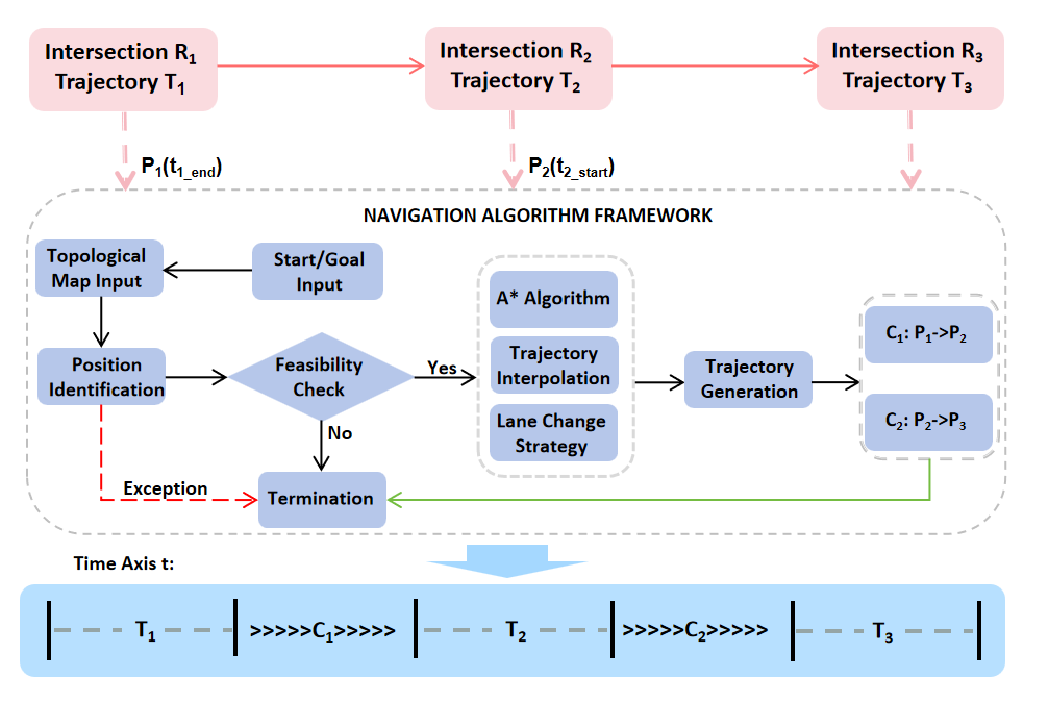
\includegraphics[width=\columnwidth]{picture/picture5.eps}}
	\caption{Trajectory restoration diagram, showing how to generate predicted trajectories between intersections from multi-object tracking trajectories and then obtain the complete vehicle trajectory.} 
	\label{fig:5} 
\end{figure}

\subsection{Twin of Trajectory}

Through the previous steps, we have obtained the trajectories of all vehicles. 
Here, we will further optimize these trajectories using a trajectory smoothing algorithm, and then employ a PID controller to control the vehicles, ensuring they follow the optimized trajectories\cite{Alpher22d}. 

A trajectory smoothing method based on linear interpolation is adopted in this work.
Given the original trajectory point set \(W = \{w_1,w_2 ,…,w_n\}\), where \(w_i \in R^2\) represents the coordinates of the \(i\)-th track point, the smoothed track \(\widetilde{W}\) is generated by:
\begin{align}
	\widetilde{W} = \bigcup_{i = 1}^{n-1} \left( w_i \cup \left\{ w_i + k\delta \cdot \frac{w_{i+1} - w_i}{d_i} \ \middle|\ k \in \mathbb{N}^+\right\} \right)
\end{align}
Precise control of trajectory density is achieved through a step size parameter \(\delta\) in this method, which maintains strict adherence to the original trajectory geometry and ensures all interpolation points are positioned on line segments connecting adjacent original waypoints.
Specifically, for any adjacent waypoint pair, the algorithm uniformly inserts new waypoints on its connection line. The number of insertion points is dynamically determined by the ratio of distance \(d_i\) to step \(\delta\), and the constraint \(k\delta < d_i\) is satisfied, thereby ensuring the adaptive matching of the interpolation density and the local geometric features of the trajectory.
It is worth noting that the current method assumes that the input waypoints are all on the real trajectory, and for the filtering of possible external or noise points, an additional robust processing mechanism is needed, which will be an important direction for future research.

This study employed a PID controller rather than more advanced control approaches such as model predictive control (MPC).
The control methods we use can be replaced by updated methods in the future.
Compared to optimization-based approaches, PID controllers offer interpretable control behavior, greater sensitivity to time delays and synchronization errors, and ensure repeatable baseline testing across diverse deployment environments.
Therefore, PID served as an effective and representative control scheme for validating the proposed digital twin mechanism.
%The PID controller consists of three main components: Proportional control (P), Integral control (I), and Derivative control (D). Each component serves a specific purpose, enabling the regulation of different aspects of the system.
\begin{align}
	u = K_p e + K_i \int \left( e - \frac{\text{sat}(u)-u}{K_p} \right) dt + K_d \dot{e}
\end{align}
This study proposes an improved PID control algorithm, whose control output \(u\) consists of proportional term, anti-saturation integral term, and differential term, where \(K_p\), \(K_i\) and \(K_d\) are proportional gain, integral gain and differential gain respectively.
The algorithm achieves rapid error response through the proportional term, eliminates steady-state errors using the integral term, and suppresses the error change rate through the differential term.
Experimental studies have shown that traditional PID control has an integral saturation phenomenon in the vehicle steering system, resulting in random extreme deflections of the steering wheel (±1 rad).
To this end, this algorithm introduces a compensation term, and the saturation function \(\text{sat}(u)\) limits the controller output \(u\) to a preset interval [\(u_{min}\), \(u_{max}\)].
When the control output reaches the saturation limit, the integral accumulation rate is automatically adjusted, which effectively solves the integral saturation problem.
\textcolor{red}{Here, \(e\) represents the error between the target value and the current system output, and \(\dot{e}\) denotes the rate of change of this error over time.}

\subsection{Evaluation}

We employed three evaluation metrics to validate the effectiveness of UTDT from perception, association, and digital twin perspectives.
Specifically, the single-intersection metric evaluates local perception accuracy, the cross-intersection metric assesses temporal and identity consistency across scenes, and the digital twin metric measures how accurately the virtual system reproduces real-world traffic dynamics.

\textbf{Multiple Object Tracking Accuracy.}
Single-camera, multi-object tracking performance is typically measured by the Multiple Object Tracking Accuracy \((MOTA)\) and Multi-Object Tracking Precision \((MOTP)\)\cite{Alpher23b}.
We use an improved evaluation metric Robust Multi-Object Tracking Accuracy \((RMOTA)\) based on sliding window median statistics, which aims to enhance the robustness of traditional \(MOTA\) to short-term occlusion and ID switching.
The tracking sequence is divided into \(W\) time windows, and each window independently calculates the local \(MOTA\) score to avoid the serious error of a single frame affecting the overall evaluation.
In addition, the penalty for identity mismatching is amplified by the coefficient \(\alpha\) to reflect the key impact of ID continuity on tracking quality.
To mitigate the impact of low-quality matches on the results, we introduce matching weights \(w_{t,i}\) on top of the original \(MOTP\).
This weighted average of the errors \(d_{t,i}\) for each match in each frame yields the weighted robust multi-object tracking precision.
The weights can be taken as detector confidence, allowing \(RMOTP\) to prioritize high-quality matches.
\begin{align}
	RMOTA = \underset{i=1}{\overset{W}{\mathrm{median}}} \left(1 - \frac{FN^{(i)} + FP^{(i)} + \alpha M^{(i)}}{T^{(i)}}\right) 
\end{align}
Among them,
\(FN^{(i)}\) (False Negatives) represents the number of missed detections in the \(i\)-th window, which means targets that truly exist but were not detected.
\(FP^{(i)}\) (False Positives) represents the number of false detections in the \(i\)-th window, which means targets that were detected but do not actually exist.
\(M^{(i)}\) (Mismatches) represents the number of identity mismatches in the \(i\)-th window, which means cases where the tracking ID of a target was incorrectly assigned during the tracking process.
\(T^{(i)}\) (Total Number of True Detections) represents the total number of true detections in the \(i\)-th window, which means the number of targets correctly detected across all frames.

\textbf{Cross-Sensor Tracking Accuracy.}
Multi-Camera Object Tracking Accuracy \((MCTA)\)\cite{Alpher23b} condenses all aspects of system performance into a metric that measures cross-camera tracking.
On this basis, this paper proposes an Interpretable Multi-Intersection Object Tracking Accuracy \((MITA)\), which is defined as follows:
\begin{align}
	MITA = {\frac{2PR}{P + R}}_{\text{}} \times \prod_{k \in \{w, h\}} \left(1 - \frac{M_k + \lambda E_k^{\text{ID}}}{T_k}\right)
\end{align}
by decomposing the cross-camera error into missing association \(M_k\) and ID switching \(E_k^{\text{ID}}\), accurate diagnosis of system defects is achieved.
Among them,
\(P\) represents the proportion of correct matches (correctly identifying and tracking targets) across all cameras.  
\(R\) represents the recall rate, which is the proportion of all true targets that are correctly tracked.  
\(\lambda\) is the penalty coefficient for ID switching error and \(T_k\) represents the total number of potential correct associations in the \(k\)-th dimension, and \(w\) and \(h\) represent within-intersection and between-intersection, respectively.

Compared with \(MCTA\), \(MITA\) intuitively demonstrates the independent evaluation and synergy of detection capability and cross-camera association capability, transforming complex cross-camera evaluation into a transparent framework that is quantifiable, adjustable, and diagnosable.
%\begin{table*}[t]
%	\centering
%	\renewcommand{\arraystretch}{1.3}
%	\caption{MULTI-OBJECTIVE TRACKING EVALUATION}
%	\label{tab:2}
%	\small
%	\setlength{\tabcolsep}{3.5pt}
%	\begin{tabular}{@{}p{1.6cm}@{\hspace{1.2em}}c@{\hspace{0.15em}}*{9}{c}@{}}
%		\toprule
%		\textbf{Scene} & \textbf{Int.} & \makebox[1.5cm][c]{\textbf{Rcll}} & \makebox[1.5cm][c]{\textbf{Prcn}} & \makebox[1.5cm][c]{\textbf{FTR}} & \makebox[0.7cm][c]{\textbf{FN}} & \textbf{IDS} & \makebox[1.5cm][c]{\textbf{MT}} & \makebox[1.5cm][c]{\textbf{ML}} & \makebox[1.5cm][c]{\textbf{RMOTA}} & \makebox[1.5cm][c]{\textbf{RMOTP}} \\
%		\midrule
%		\multirow{5}{*}{\shortstack[l]{Town01 \\ (16 ints., flat \\ roads, sparsely \\ populated buil- \\ dings)}}
%		& 1 & \textcolor{red}{$26.69 \pm 3.34$} & \textcolor{red}{$69.19 \pm 1.41$} & \textcolor{red}{$0.30 \pm 0.06$} & \textcolor{red}{787} & \textcolor{red}{18} & \textcolor{red}{$0.00 \pm 0.00$} & \textcolor{red}{$37.5 \pm 0.00$} & \textcolor{red}{$13.08 \pm 0.59$} & \textcolor{red}{$80.58 \pm 0.25$} \\
%		& 2 & \textcolor{red}{$63.21 \pm 3.20$} & \textcolor{red}{$63.08 \pm 3.44$} & \textcolor{red}{$0.95 \pm 0.17$} & \textcolor{red}{409} & \textcolor{red}{17} & \textcolor{red}{$50.00 \pm 11.11$} & \textcolor{red}{$33.33 \pm 0.00$} & \textcolor{red}{$24.30 \pm 4.39$} & \textcolor{red}{$87.02 \pm 0.48$} \\
%		& 3 & \textcolor{red}{$59.88 \pm 6.10$} & \textcolor{red}{$44.78 \pm 1.36$} & \textcolor{red}{$1.19 \pm 0.06$} & \textcolor{red}{190} & \textcolor{red}{11} & \textcolor{red}{$0.00 \pm 0.00$} & \textcolor{red}{$25.00 \pm 0.00$} & \textcolor{red}{$-16.97 \pm 0.90$} & \textcolor{red}{$87.13 \pm 0.33$} \\
%		& 4 & \textcolor{red}{$61.93 \pm 6.67$} & \textcolor{red}{$97.20 \pm 0.60$} & \textcolor{red}{$0.03 \pm 0.00$} & \textcolor{red}{225} & \textcolor{red}{26} & \textcolor{red}{$35.00 \pm 10.00$} & \textcolor{red}{$20.00 \pm 0.00$} & \textcolor{red}{$56.81 \pm 5.96$} & \textcolor{red}{$89.15 \pm 0.16$} \\
%		& 5 & \textcolor{red}{$37.11 \pm 4.25$} & \textcolor{red}{$94.07 \pm 2.83$} & \textcolor{red}{$0.03 \pm 0.02$} & \textcolor{red}{149} & \textcolor{red}{11} & \textcolor{red}{$50.00 \pm 0.00$} & \textcolor{red}{$50.00 \pm 0.00$} & \textcolor{red}{$30.96 \pm 2.92$} & \textcolor{red}{$88.43 \pm 0.11$} \\
%		
%%		\addlinespace
%		\multirow{5}{*}{\shortstack[l]{Town10 \\ (7 ints., high- \\ density, inclu- \\ ding steep slo- \\ pes)}} 		
%		& 1 & \textcolor{red}{$29.50 \pm 2.37$} & \textcolor{red}{$60.37 \pm 1.28$} & \textcolor{red}{$0.80 \pm 0.00$} & \textcolor{red}{1334} & \textcolor{red}{25} & \textcolor{red}{$8.33 \pm 0.00$} & \textcolor{red}{$50.00 \pm 0.00$} & \textcolor{red}{$8.80 \pm 0.69$} & \textcolor{red}{$84.90 \pm 0.49$} \\
%		& 2 & \textcolor{red}{$54.53 \pm 3.87$} & \textcolor{red}{$71.47 \pm 3.16$} & \textcolor{red}{$1.07 \pm 0.22$} & \textcolor{red}{1101} & \textcolor{red}{22} & \textcolor{red}{$10.00 \pm 6.67$} & \textcolor{red}{$11.11 \pm 3.33$} & \textcolor{red}{$31.56 \pm 1.44$} & \textcolor{red}{$81.23 \pm 0.37$} \\
%		& 3 & \textcolor{red}{$50.71 \pm 1.91$} & \textcolor{red}{$78.56 \pm 5.21$} & \textcolor{red}{$0.52 \pm 0.17$} & \textcolor{red}{908} & \textcolor{red}{15} & \textcolor{red}{$16.67 \pm 4.12$} & \textcolor{red}{$35.71 \pm 0.00$} & \textcolor{red}{$35.78 \pm 2.80$} & \textcolor{red}{$84.61 \pm 0.22$} \\
%		& 4 & \textcolor{red}{$49.50 \pm 5.39$} & \textcolor{red}{$86.59 \pm 0.60$} & \textcolor{red}{$0.25 \pm 0.04$} & \textcolor{red}{806} & \textcolor{red}{42} & \textcolor{red}{$24.99 \pm 4.55$} & \textcolor{red}{$36.36 \pm 0.00$} & \textcolor{red}{$39.21 \pm 3.17$} & \textcolor{red}{$88.66 \pm 0.13$} \\
%		& 5 & \textcolor{red}{$43.61 \pm 3.67$} & \textcolor{red}{$63.73 \pm 3.00$} & \textcolor{red}{$1.51 \pm 0.30$} & \textcolor{red}{1695} & \textcolor{red}{27} & \textcolor{red}{$9.38 \pm 6.25$} & \textcolor{red}{$37.50 \pm 0.00$} & \textcolor{red}{$17.58 \pm 1.79$} & \textcolor{red}{$86.21 \pm 0.26$} \\
%		
%%		\addlinespace
%		\multirow{2}{*}{\textcolor{red}{\shortstack[l]{CEC Software \\ Park(7 ints.)}}} 
%		& \textcolor{red}{1} & \textcolor{red}{$39.67 \pm 5.52$} & \textcolor{red}{$51.40 \pm 1.23$} & \textcolor{red}{$0.94 \pm 0.17$} & \textcolor{red}{460} & \textcolor{red}{18} & \textcolor{red}{$16.67 \pm 0.00$} & \textcolor{red}{$38.89 \pm 9.62$} & \textcolor{red}{$-0.44 \pm 1.97$} & \textcolor{red}{$69.69 \pm 0.51$} \\
%		& \textcolor{red}{2} & \textcolor{red}{$64.22 \pm 4.35$} & \textcolor{red}{$55.48 \pm 1.94$} & \textcolor{red}{$1.11 \pm 0.16$} & \textcolor{red}{181} & \textcolor{red}{4} & \textcolor{red}{$52.38 \pm 8.25$} & \textcolor{red}{$17.29 \pm 0.00$} & \textcolor{red}{$11.68 \pm 3.09$} & \textcolor{red}{$83.90 \pm 0.57$} \\
%		\bottomrule
%	\end{tabular}
%\end{table*}
\begin{table*}[t]
	\centering
	\renewcommand{\arraystretch}{1.3}
	\caption{MULTI-OBJECTIVE TRACKING EVALUATION}
	\label{tab:2}
	\small
	\setlength{\tabcolsep}{3.5pt}
	\begin{tabular}{@{}p{1.6cm}@{\hspace{1.2em}}c@{\hspace{0.15em}}*{9}{c}@{}}
		\toprule
		\textbf{Scene} & \textbf{Int.} & \makebox[1.5cm][c]{\textbf{Rcll}} & \makebox[1.5cm][c]{\textbf{Prcn}} & \makebox[1.5cm][c]{\textbf{FTR}} & \makebox[0.7cm][c]{\textbf{FN}} & \textbf{IDS} & \makebox[1.5cm][c]{\textbf{MT}} & \makebox[1.5cm][c]{\textbf{ML}} & \makebox[1.5cm][c]{\textbf{RMOTA}} & \makebox[1.5cm][c]{\textbf{RMOTP}} \\
		\midrule
		\multirow{5}{*}{\shortstack[l]{Town01 \\ (16 ints., flat \\ roads, sparsely \\ populated buil- \\ dings)}}
		& 1 & $26.69 \pm 3.34$ & $69.19 \pm 1.41$ & $0.30 \pm 0.06$ & 787 & 18 & $0.00 \pm 0.00$ & $37.5 \pm 0.00$ & $13.08 \pm 0.59$ & $80.58 \pm 0.25$ \\
		& 2 & $63.21 \pm 3.20$ & $63.08 \pm 3.44$ & $0.95 \pm 0.17$ & 409 & 17 & $50.00 \pm 11.11$ & $33.33 \pm 0.00$ & $24.30 \pm 4.39$ & $87.02 \pm 0.48$ \\
		& 3 & $59.88 \pm 6.10$ & $44.78 \pm 1.36$ & $1.19 \pm 0.06$ & 190 & 11 & $0.00 \pm 0.00$ & $25.00 \pm 0.00$ & $-16.97 \pm 0.90$ & $87.13 \pm 0.33$ \\
		& 4 & $61.93 \pm 6.67$ & $97.20 \pm 0.60$ & $0.03 \pm 0.00$ & 225 & 26 & $35.00 \pm 10.00$ & $20.00 \pm 0.00$ & $56.81 \pm 5.96$ & $89.15 \pm 0.16$ \\
		& 5 & $37.11 \pm 4.25$ & $94.07 \pm 2.83$ & $0.03 \pm 0.02$ & 149 & 11 & $50.00 \pm 0.00$ & $50.00 \pm 0.00$ & $30.96 \pm 2.92$ & $88.43 \pm 0.11$ \\
		
		\multirow{5}{*}{\shortstack[l]{Town10 \\ (7 ints., high- \\ density, inclu- \\ ding steep slo- \\ pes)}} 		
		& 1 & $29.50 \pm 2.37$ & $60.37 \pm 1.28$ & $0.80 \pm 0.00$ & 1334 & 25 & $8.33 \pm 0.00$ & $50.00 \pm 0.00$ & $8.80 \pm 0.69$ & $84.90 \pm 0.49$ \\
		& 2 & $54.53 \pm 3.87$ & $71.47 \pm 3.16$ & $1.07 \pm 0.22$ & 1101 & 22 & $10.00 \pm 6.67$ & $11.11 \pm 3.33$ & $31.56 \pm 1.44$ & $81.23 \pm 0.37$ \\
		& 3 & $50.71 \pm 1.91$ & $78.56 \pm 5.21$ & $0.52 \pm 0.17$ & 908 & 15 & $16.67 \pm 4.12$ & $35.71 \pm 0.00$ & $35.78 \pm 2.80$ & $84.61 \pm 0.22$ \\
		& 4 & $49.50 \pm 5.39$ & $86.59 \pm 0.60$ & $0.25 \pm 0.04$ & 806 & 42 & $24.99 \pm 4.55$ & $36.36 \pm 0.00$ & $39.21 \pm 3.17$ & $88.66 \pm 0.13$ \\
		& 5 & $43.61 \pm 3.67$ & $63.73 \pm 3.00$ & $1.51 \pm 0.30$ & 1695 & 27 & $9.38 \pm 6.25$ & $37.50 \pm 0.00$ & $17.58 \pm 1.79$ & $86.21 \pm 0.26$ \\
		
		\multirow{2}{*}{\shortstack[l]{CEC Software \\ Park (7 ints.)}} 
		& 1 & $39.67 \pm 5.52$ & $51.40 \pm 1.23$ & $0.94 \pm 0.17$ & 460 & 18 & $16.67 \pm 0.00$ & $38.89 \pm 9.62$ & $-0.44 \pm 1.97$ & $69.69 \pm 0.51$ \\
		& 2 & $64.22 \pm 4.35$ & $55.48 \pm 1.94$ & $1.11 \pm 0.16$ & 181 & 4 & $52.38 \pm 8.25$ & $17.29 \pm 0.00$ & $11.68 \pm 3.09$ & $83.90 \pm 0.57$ \\
		\bottomrule
	\end{tabular}
\end{table*}

\textbf{Twin Accuracy.}
In the twin experimental evaluation, we verify the effectiveness of the system by comparing the comprehensive performance of the following three key trajectories: (1) the actual trajectory of the vehicle, (2) the observed trajectory reconstructed based on the multi-object tracking algorithm, and (3) the expected trajectory generated by the control system.
This study uses Trajectory Overlap Ratio \((TOR)\) for comprehensive evaluation, which quantifies both the shape similarity of the trajectory and the spatiotemporal consistency of the waypoints.
\begin{align}
	TOR & = \left(1 - \frac{D_{dtw}}{D_{max}}\right) \times \Lambda(\tau)
\end{align}
Among them, the shape similarity term is calculated based on the ratio of the dynamic time warping distance \(D_{dtw}\) to the maximum scale distance \(D_{max}\), reflecting the overall geometric difference of the trajectory, while the spatial alignment term \(\Lambda(\tau)\) evaluates the static matching accuracy of the waypoint through the position offset penalty.
This evaluation mechanism can not only capture the morphological differences of macroscopic paths, but also characterize the spatiotemporal consistency of discrete waypoints at the micro level, providing a multi-dimensional quantitative basis for the trajectory consistency of the digital twin system.
\begin{align}
	D_{dtw} = \min_{\pi \in P} \sqrt{\sum_{(i,j)\in\pi} \|p_i - q_j\|^2}
\end{align}
\begin{align}
	D_{max} = \max_{i,j} \|p_i - q_j\| \cdot \max(n,m)
\end{align}
\(D_{dtw}\) compares the similarity of non-aligned sequences through a dynamic curved path \(\pi\), and finds the matching solution that minimizes the cumulative distance from all possible path sets \(P\), while \(D_{max}\) quantifies the spatial deviation of the two trajectories in the worst case and normalizes it by the trajectory length. Among them, \(p_{i}\) and \(p_{j}\) represent the matching point pairs of the two trajectories, and \(m\) and \(n\) are the lengths of the two trajectories respectively.

\begin{align}
	\Lambda(\tau) = \frac{1}{n} \sum_{k=1}^{n} \mathbb{I}\left(\left\|p_{\pi_{1}(k)}-q_{\pi_{2}(k)}\right\| \leq \tau\right)
\end{align}
The trajectory we finally get is the coordinates in the simulation scenario, which means that the trajectory is actually discrete.
Therefore, calculating the positional relationship between waypoints is very important to reflect the overlap between two trajectories.
\(\Lambda(\tau)\) counts the proportion of matching points in the two trajectories whose distance is less than the threshold \(\tau\) to reflect the overlap accuracy of the two trajectories within the allowable error range.
where \(p_{\pi_{1}(k)}\) and \(q_{\pi_{2}(k)}\) represent the three-dimensional coordinates of the \(\pi_{1}(k)\)th point of trajectory 1 and the \(\pi_{2}(k)\)th point of trajectory 2, respectively, and \(\mathbb{I}(\cdot)\) is the indicator function (which takes the value of 1 when the Euclidean distance between two points does not exceed the threshold \(\tau\), otherwise it takes the value of 0).
%\begin{table*}[t]
%	\centering
%	\caption{Performance Comparison of Trajectory and Vehicle Control Indicators}
%	\label{tab:3}
%	\renewcommand\arraystretch{1.3} % 微调行高,使其更紧凑
%	\begin{tabular}{@{} l l cccc ccc @{}} % 去除所有竖线 | ;使用 @{} 减少表格两侧的空白
%		\toprule % 顶部的粗线
%		\multirow{2}{*}{\textbf{Scene}} & 
%		\multirow{2}{*}{\textbf{Type}} & 
%		\multicolumn{4}{c}{\textbf{Trajectory Indicators}} & 
%		\multicolumn{3}{c}{\textbf{Control Indicators}} \\
%		% \cmidrule 用于绘制表头下的短横线,(lr) 表示线段的左右两端缩短,视觉上更美观
%		%\cmidrule(lr){3-6} \cmidrule(l){7-9}
%%		\addlinespace 
%		& & \textbf{TOR(\%)} & \textbf{MPE(m)} & \textbf{MaxPE(m)} & \textbf{FPE(m)} & \textbf{MLE(m)} & \textbf{MLOE(m)} & \textbf{MD(ms)} \\
%		\midrule % 表头与数据之间的粗线
%		\multirow{3}{*}{Town01} 
%		& TT-DT & \textcolor{red}{$47.03 \pm 0.64$} & \textcolor{red}{$16.74 \pm 0.13$} & \textcolor{red}{$33.06 \pm 0.05$} & \textcolor{red}{$26.19 \pm 3.11$} & \textcolor{red}{--} & \textcolor{red}{--} & \textcolor{red}{--} \\
%		& TT-GT & \textcolor{red}{$44.29 \pm 3.14$} & \textcolor{red}{$33.22 \pm 0.02$} & \textcolor{red}{$42.96 \pm 0.05$} & \textcolor{red}{$42.86 \pm 0.09$} & \textcolor{red}{--} & \textcolor{red}{--} & \textcolor{red}{--} \\
%		& Control & \textcolor{red}{--} & \textcolor{red}{--} & \textcolor{red}{--} & \textcolor{red}{--} & \textcolor{red}{$1.80 \pm 0.06$} & \textcolor{red}{$0.84 \pm 0.11$} & \textcolor{red}{$0.61 \pm 0.10$} \\
%%
%%		\addlinespace % 数据组之间的分隔线
%		\multirow{3}{*}{Town10} 
%		& TT-DT & \textcolor{red}{$22.11 \pm 0.08$} & \textcolor{red}{$81.92 \pm 0.47$} & \textcolor{red}{$85.03 \pm 0.87$} & \textcolor{red}{$51.65 \pm 2.72$} & \textcolor{red}{--} & \textcolor{red}{--} & \textcolor{red}{--} \\
%		& TT-GT & \textcolor{red}{$48.25 \pm 0.39$} & \textcolor{red}{$52.41 \pm 0.01$} & \textcolor{red}{$101.94 \pm 0.20$} & \textcolor{red}{$52.99 \pm 0.02$} & \textcolor{red}{--} & \textcolor{red}{--} & \textcolor{red}{--} \\
%		& Control & \textcolor{red}{--} & \textcolor{red}{--} & \textcolor{red}{--} & \textcolor{red}{--} & \textcolor{red}{$0.98 \pm 0.35$} & \textcolor{red}{$0.45 \pm 0.03$} & \textcolor{red}{$1.78 \pm 0.06$} \\
%%
%%		\addlinespace % 数据组之间的分隔线
%		\multirow{3}{*}{\textcolor{red}{\shortstack[l]{CEC Soft- \\ware Park}}} 
%        & \textcolor{red}{TT-DT} & \textcolor{red}{$22.23 \pm 1.01$} & \textcolor{red}{$212.86 \pm 32.14$} & \textcolor{red}{$199.49 \pm 27.25$} & \textcolor{red}{$196.68 \pm 28.68$} & \textcolor{red}{--} & \textcolor{red}{--} & \textcolor{red}{--} \\
%		& \textcolor{red}{TT-GT} & \textcolor{red}{$8.82 \pm 0.03$} & \textcolor{red}{$176.68 \pm 14.13$} & \textcolor{red}{$205.30 \pm 14.15$} & \textcolor{red}{$174.89 \pm 14.18$} & \textcolor{red}{--} & \textcolor{red}{--} & \textcolor{red}{--} \\
%		& \textcolor{red}{Control} & \textcolor{red}{--} & \textcolor{red}{--} & \textcolor{red}{--} & \textcolor{red}{--} & \textcolor{red}{$1.58 \pm 0.17$} & \textcolor{red}{$0.53 \pm 0.05$} & \textcolor{red}{$1.25 \pm 0.31$} \\
%		\bottomrule % 底部的粗线·
%	\end{tabular}
%\end{table*}
\begin{table*}[t]
	\centering
	\caption{Performance Comparison of Trajectory and Vehicle Control Indicators}
	\label{tab:3}
	\renewcommand\arraystretch{1.3} % 微调行高,使其更紧凑
	\begin{tabular}{@{} l l cccc ccc @{}} 
		\toprule
		\multirow{2}{*}{\textbf{Scene}} & 
		\multirow{2}{*}{\textbf{Type}} & 
		\multicolumn{4}{c}{\textbf{Trajectory Indicators}} & 
		\multicolumn{3}{c}{\textbf{Control Indicators}} \\
		& & \textbf{TOR(\%)} & \textbf{MPE(m)} & \textbf{MaxPE(m)} & \textbf{FPE(m)} & \textbf{MLE(m)} & \textbf{MLOE(m)} & \textbf{MD(ms)} \\
		\midrule
		\multirow{3}{*}{Town01} 
		& TT-DT & $47.03 \pm 0.64$ & $16.74 \pm 0.13$ & $33.06 \pm 0.05$ & $26.19 \pm 3.11$ & -- & -- & -- \\
		& TT-GT & $44.29 \pm 3.14$ & $33.22 \pm 0.02$ & $42.96 \pm 0.05$ & $42.86 \pm 0.09$ & -- & -- & -- \\
		& Control & -- & -- & -- & -- & $1.80 \pm 0.06$ & $0.84 \pm 0.11$ & $0.61 \pm 0.10$ \\
		
		\multirow{3}{*}{Town10} 
		& TT-DT & $22.11 \pm 0.08$ & $81.92 \pm 0.47$ & $85.03 \pm 0.87$ & $51.65 \pm 2.72$ & -- & -- & -- \\
		& TT-GT & $48.25 \pm 0.39$ & $52.41 \pm 0.01$ & $101.94 \pm 0.20$ & $52.99 \pm 0.02$ & -- & -- & -- \\
		& Control & -- & -- & -- & -- & $0.98 \pm 0.35$ & $0.45 \pm 0.03$ & $1.78 \pm 0.06$ \\
		
		\multirow{3}{*}{\shortstack[l]{CEC Soft- \\ware Park}} 
		& TT-DT & $22.23 \pm 1.01$ & $212.86 \pm 32.14$ & $199.49 \pm 27.25$ & $196.68 \pm 28.68$ & -- & -- & -- \\
		& TT-GT & $8.82 \pm 0.03$ & $176.68 \pm 14.13$ & $205.30 \pm 14.15$ & $174.89 \pm 14.18$ & -- & -- & -- \\
		& Control & -- & -- & -- & -- & $1.58 \pm 0.17$ & $0.53 \pm 0.05$ & $1.25 \pm 0.31$ \\
		\bottomrule
	\end{tabular}
\end{table*}

\section{Experiments}

\subsection{Preparation}

\textbf{Simulation Environment.}
We conducted simulation experiments in CARLA, whose advantage lies in its provision of a highly realistic virtual environment capable of accurately simulating complex traffic scenarios and diverse driving conditions. 
CARLA supports flexible sensor configurations, such as cameras and LiDAR, facilitating multimodal data acquisition and fusion experiments\cite{Alpher22e}. 
We conducted relevant experiments in the Town10 and Town01 scenarios in CARLA.
The complex urban structure and dense traffic flow of Town10 can simulate highly dynamic real traffic environments, while the simple layout and clear rules of Town01 make it easy to construct controlled experimental scenarios.
This scenario diversity can effectively verify the generalization ability of the model under different traffic conditions and provide a reliable basis for actual road deployment.

\textbf{Data Collection.}
In CARLA's Town10 scenario, a single intersection location is selected, with a LiDAR placed at the center and six cameras arranged around it to achieve 360-degree omnidirectional perception coverage. 
In our configuration, the heights of the lidar and camera relative to the ego vehicle are \(h_{LE}\) (0.82 m) and \(h_{C}\) (2.62 m), respectively. 
On the front and rear sides of the vehicle, the lateral spacing between the three cameras on each side is \(d_{CC}\) (4 m), and the lidar is located between the cameras on the front and rear sides of the vehicle, and the horizontal distance from the front and rear cameras is \(d_{LC}\) (7 m).
The same 64-line LiDAR (range measurement: 200m, point cloud density: 2.2M pts/s, scanning frequency: 20Hz) configuration as that used for collecting PointPillars network training data is used, and a wide-angle camera with a resolution of 1920\(\times\)1080 pixels and a field of view of 90\(\degree\) is deployed simultaneously to achieve multimodal collection of point cloud and high-definition image data.
The data structure follows the storage format of the Panda dataset, making the data more standardized for subsequent processing and fusion\cite{Alpher21c}.

\subsection{Experimental Effect}

\textbf{Multi-Object Tracking.}
Table \ref{tab:2} presents the multi-object tracking performance metrics across different scenarios, including five intersections in the simulated environments (Town01 and Town10) and two real-world intersections in the CEC Software Park.
The data reveals significant variations in performance across different intersections. 
In Town01, Intersection 4 shows better performance in terms of Recall and Precision, while Intersection 3 has a higher False Track Ratio (FTR), indicating a greater proportion of incorrect tracking. 
In Town10, Intersection 4 also demonstrates relatively high Recall and Precision, but Intersection 5 has significantly higher False Negatives (FN) compared to other intersections, suggesting a higher number of missed targets. 
Identity Switches (IDS) are notably higher in Intersection 4 of both Town01 and Town10, indicating more frequent target identity switches at these intersections. 
Intersection 2 (Town01) shows higher Mostly Tracked (MT), while Intersection 1 (Town10) has higher Mostly Lost (ML), indicating notable tracking stability differences.
CEC Software Park's multi-object tracking performance is slightly lower than that of the simulated scenarios Town01 and Town10, mainly in terms of target detection accuracy and trajectory matching accuracy (especially at the first intersection). However, the recall rate remains at a similar level, demonstrating that the algorithm remains robust and transferable under real-world perceptual noise.

%\begin{table*}[t]
%	\centering
%	\caption{\textcolor{red}{Multi-Objective Tracking Evaluation Under Extreme Weather Conditions}}
%	\label{tab:6}
%	\small
%	\renewcommand{\arraystretch}{1.5}  % 增加行距
%	\begin{tabular}{l cccccccccccc}
%		\toprule
%		\textcolor{red}{\textbf{Weather}} & \textcolor{red}{\textbf{Vehicle}} & \textcolor{red}{\textbf{AAC}} & \textcolor{red}{\textbf{Rcll}} & \textcolor{red}{\textbf{Prcn}} & \textcolor{red}{\textbf{FTR}} & \textcolor{red}{\textbf{FP}} & \textcolor{red}{\textbf{FN}} & \textcolor{red}{\textbf{IDS}} & \textcolor{red}{\textbf{MT}} & \textcolor{red}{\textbf{ML}} & \textcolor{red}{\textbf{RMOTA}} & \textcolor{red}{\textbf{RMOTP}} \\
%		\midrule
%		\textcolor{red}{\raggedright Clear} & \textcolor{red}{50}  & \textcolor{red}{0.0004} & \textcolor{red}{24.67} & \textcolor{red}{63.61} & \textcolor{red}{0.32} & \textcolor{red}{139} & \textcolor{red}{742}  & \textcolor{red}{6}  & \textcolor{red}{20.00} & \textcolor{red}{50.00} & \textcolor{red}{9.95}  & \textcolor{red}{87.14} \\
%		\textcolor{red}{\raggedright Clear} & \textcolor{red}{150} & \textcolor{red}{0.0004} & \textcolor{red}{41.99} & \textcolor{red}{88.48} & \textcolor{red}{0.63} & \textcolor{red}{313} & \textcolor{red}{3319} & \textcolor{red}{41} & \textcolor{red}{28.57} & \textcolor{red}{50.00} & \textcolor{red}{35.81} & \textcolor{red}{84.83} \\
%		\textcolor{red}{\raggedright Rainy} & \textcolor{red}{50}  & \textcolor{red}{0.0644} & \textcolor{red}{8.02}  & \textcolor{red}{54.48} & \textcolor{red}{0.15} & \textcolor{red}{66}  & \textcolor{red}{906}  & \textcolor{red}{15} & \textcolor{red}{10.00} & \textcolor{red}{60.00} & \textcolor{red}{-0.20} & \textcolor{red}{79.02} \\
%		\textcolor{red}{\raggedright Foggy} & \textcolor{red}{50}  & \textcolor{red}{1.0416} & \textcolor{red}{3.05}  & \textcolor{red}{33.71} & \textcolor{red}{0.14} & \textcolor{red}{59}  & \textcolor{red}{955}  & \textcolor{red}{11} & \textcolor{red}{20.00} & \textcolor{red}{80.00} & \textcolor{red}{-4.06} & \textcolor{red}{71.99} \\
%		\bottomrule
%	\end{tabular}
%\end{table*}


\begin{table}[t]
	\centering
	\caption{Twin Accuracy Comparison Across Detection Algorithms}
	\label{tab:5}
	\renewcommand\arraystretch{1.2}
	\resizebox{\columnwidth}{!}{ 
		\begin{tabular}{l l cccc}
			\toprule
			\textbf{Detection} & \textbf{Type} & \textbf{TOR(\%)} & \textbf{MPE(m)} & \textbf{MaxPE(m)} & \textbf{FPE(m)} \\
			\midrule
			\multirow{2}{*}{LiDAR} 
			& TT-DT & 9.99 & 93.10 & 107.39 & 102.10 \\
			& TT-GT & 28.98 & 33.88 & 35.10 & 35.10 \\
%			\addlinespace
			\multirow{2}{*}{Camera} 
			& TT-DT & -- & -- & -- & -- \\
			& TT-GT & -- & -- & -- & -- \\
%			\addlinespace
			\multirow{2}{*}{YOLOv3+LiDAR} 
			& TT-DT & 10.09 & 98.21 & 100.62 & 98.72 \\	
			& TT-GT & 31.90 & 78.64 & 102.47 & 59.67 \\
%			\addlinespace
			\multirow{2}{*}{YOLOv4+LiDAR} 
			& TT-DT & 42.11 & 81.92 & 85.03 & 51.65 \\
			& TT-GT & 48.25 & 52.41 & 101.94 & 52.99 \\
			\bottomrule
		\end{tabular}
	}
\end{table}

%\begin{table}[t]
%	\centering
%	\caption{\textcolor{red}{Town10: RMOTA and RMOTP comparison between UTDT and DeepSORT}}
%	\label{tab:7}
%	\renewcommand\arraystretch{1.2}
%	\begin{tabular}{c c c c c}
%		\toprule
%		\multirow{2}{*}{\textcolor{red}{Int.}} & \multicolumn{2}{c}{\textcolor{red}{RMOTA}} & \multicolumn{2}{c}{\textcolor{red}{RMOTP}} \\
%		\cmidrule(lr){2-3} \cmidrule(lr){4-5}
%		& \textcolor{red}{UTDT} & \textcolor{red}{DeepSORT} & \textcolor{red}{UTDT} & \textcolor{red}{DeepSORT} \\
%		\midrule
%		1 & \textcolor{red}{$8.80 \pm 0.69$} & \textcolor{red}{$40.92 \pm 1.09$} & \textcolor{red}{$84.90 \pm 0.49$} & \textcolor{red}{$19.27 \pm 0.17$} \\
%		2 & \textcolor{red}{$31.56 \pm 1.44$} & \textcolor{red}{$22.02 \pm 0.09$} & \textcolor{red}{$81.23 \pm 0.37$} & \textcolor{red}{$27.50 \pm 0.35$} \\
%		3 & \textcolor{red}{$35.78 \pm 2.80$} & \textcolor{red}{$31.57 \pm 0.39$} & \textcolor{red}{$84.61 \pm 0.22$} & \textcolor{red}{$25.03 \pm 0.06$} \\
%		4 & \textcolor{red}{$39.21 \pm 3.17$} & \textcolor{red}{$53.60 \pm 3.88$} & \textcolor{red}{$88.66 \pm 0.13$} & \textcolor{red}{$31.20 \pm 0.29$} \\
%		5 & \textcolor{red}{$17.58 \pm 1.79$} & \textcolor{red}{$46.87 \pm 0.28$} & \textcolor{red}{$86.21 \pm 0.26$} & \textcolor{red}{$21.87 \pm 0.22$} \\
%		\bottomrule
%	\end{tabular}
%\end{table}

%However, detection accuracy is also affected by the number of vehicles passing through the intersection, and the system accuracy improves significantly in low traffic conditions.
%These data highlight the performance variations of the multi-object tracking system across different scenarios and intersections, providing valuable insights for further optimization.

To further evaluate the robustness of the proposed multi-target tracking system, additional experiments were conducted under challenging conditions, including extreme weather (rain and fog) and high-density traffic flows.
Following the optical attenuation model described in \cite{liu2020influences}, the atmospheric attenuation coefficients (AAC) of 1550 nm LiDAR signals were calculated to simulate the effects of rainfall and haze on sensing performance. 
Specifically, the attenuation coefficients under rainfall intensity of 0.4 mm/h and haze concentration of 2.6 mg/m³ were 0.0644 and 1.0416, respectively, and were introduced into the simulation to analyze tracking accuracy degradation. 
\textcolor{red}{Meanwhile, the camera sensor model explicitly accounts for weather-induced visibility degradation, with effective visibility distances set to 1.77 km for rainy conditions and 1.5 km for foggy conditions, thereby jointly reflecting the adverse impact of extreme weather on both LiDAR and vision-based perception.}
Moreover, a high-density traffic scenario with 150 vehicles (three times the baseline) was designed to examine the algorithm’s stability under congested conditions.
%The experimental results of intersection 1 in the Town10 scene are shown in Table \ref{tab:6}.
 

\textbf{Digital Twin.}
%The performance of the digital twin is primarily evaluated using three sets of metrics: trajectory coincidence, control error, and speed correlation, which together provide a comprehensive assessment of spatial, temporal, and dynamic consistency with the real-world system (as shown in Table \ref{tab:3}).
%These metrics are compared across three scenarios: Town01, Town10, and the real-world CEC Software Park.
%The TOR in Town01 is significantly highest in the comparison of the Tracking Trajectory with the Digital Twin trajectory (TT-DT), indicating that it has a superior path tracking ability, which may be due to the simpler environment or the more stable control algorithm.
%However, for the comparison between the Tracked Trajectory and Ground Truth (TT-GT), it is highest in Town10, probably because our point cloud dataset was collected in Town10 and is more suitable for vehicle detection in this scenario.
%In terms of Mean Position Error (MPE), Town01 has a smallest error, which may also be the result of a simpler environment.
%However, the Maximum Position Error (MaxPE) and Final Position Error (FPE) in Town10 far exceed those in Town01, revealing severe localization deviations in extreme cases, likely caused by complex environments or dynamic obstacles. 
%For Mean Lateral Error (MLE) and Mean Longitudinal Error (MLOE), Town10 performs slightly better, suggesting more precise lateral and longitudinal control, though overall stability is lacking. 
%In the  CEC Software Park scenario, both MPE and extreme errors (MaxPE, FPE) are significantly higher than in the simulated towns, reflecting the challenges of complex real-world environments. Nevertheless, lateral and longitudinal control errors are comparable to Town10, while the Mean Delay (MD) is intermediate, indicating acceptable task execution efficiency despite environmental complexity.
%Within Town10, velocity estimation methods exhibit limited accuracy and stability, with a low mean correlation of 0.291 and a high standard deviation of 0.559, highlighting a key bottleneck in the dynamic tracking module.
\textcolor{red}{Digital twin performance is assessed via trajectory coincidence, control error, and spatiotemporal consistency (Table \ref{tab:3}). 
In the comparison between the tracked trajectory and the digital twin trajectory (TT-DT), Town01 achieved the highest trajectory overlap (TOR), reflecting its superior path tracking performance in simpler environments.
In contrast, for the comparison between the tracked trajectory and the real trajectory (TT-GT), Town10 reached the peak, consistent with the point cloud dataset source.
Town01 had the lowest Mean Position Error (MPE), while Town10 had higher Maximum Position Error (MaxPE) and Final Position Error (FPE), indicating localization bias in complex scenarios.
Town10 had slightly better lateral and longitudinal errors (MLE, MLOE), but its overall stability was limited.}
In the CEC Software Park, both MPE and extreme errors (MaxPE, FPE) are significantly higher than in the simulated towns, reflecting the challenges of complex real-world environments. Nevertheless, lateral and longitudinal control errors are comparable to Town10, while the Mean Delay (MD) is intermediate, indicating acceptable task execution efficiency despite environmental complexity.
\textcolor{red}{To further assess spatiotemporal consistency, additional experiments were conducted to analyze the impact of severe velocity interpolation and system latency.
A unified evaluation of position, pose, interaction, and velocity correlation was introduced to characterize digital twin coherence under dynamic delays.}

\begin{figure}[!t]
	\centering
	\centerline{\includegraphics[width=\columnwidth]{picture/picture6.eps}}
	\caption{Analysis of the impact of point cloud detection threshold on multi-object tracking performance. Experiments show that the accuracy and threshold of vehicle detection are the key factors affecting tracking performance.} 
	\label{fig:6} 
\end{figure}

\textbf{Ablation Experiment for Digital Twins.}
%In the ablation experiment, we compared the multi-object tracking performance of different object detection algorithms and different sensor combinations in the Town10 scene.
%The experimental results are shown in Table \ref{tab:5}.
%When the camera is used alone, no valid trajectory can be generated (lack of depth information), and although the LiDAR can track the target alone, the overlap between its trajectory and the real annotation is significantly lower than that of the multi-sensor fusion solution; it is worth noting that the (\(RMOTA\) of LiDAR tracking alone is better than the camera-radar fusion, which shows that the camera may introduce noise (such as view occlusion) in position tracking, but it is still indispensable in the target association stage.
%The experiment further shows that the 2D/3D fusion effect of YOLOv4/LiDAR is the best (about 8\% higher than the YOLOv3 solution), which verifies the improvement of algorithm optimization on tracking accuracy.
%These results show that although the camera will suppress the position tracking accuracy, it has an irreplaceable role in target association, and the system design needs to be optimized through sensor complementarity.
%
%We further compared the tracking performance of the proposed UTDT module and the DeepSORT baseline on the same Town10 dataset (Table \ref{tab:7}).
%The results show that DeepSORT \cite{wojke2017simple} achieves overall higher RMOTA and lower RMOTP, indicating slightly better multi-object tracking accuracy and position precision in most intersections.
%However, UTDT maintains comparable performance and remains more adaptable to complex road structures and dense traffic scenes involving steep slopes and occlusions.
%These findings suggest that while DeepSORT provides stronger frame-level tracking accuracy, the UTDT framework offers better scalability and sensor-fusion flexibility for multi-intersection digital twin applications.
\textcolor{red}{In the Town10 ablation experiment (Table \ref{tab:5}), tracking using only a camera failed due to a lack of depth information; while using LiDAR alone could generate effective trajectories, its TOR was lower than that of multi-sensor fusion.
Although the \(RMOTA\) value of LiDAR alone was higher than that of camera-LiDAR fusion (reflecting noise introduced by the camera in occlusion situations), the camera remains indispensable for target association.
YOLOv4-LiDAR fusion achieved the best performance, improving upon YOLOv3 by approximately 8\%.
We further compared UTDT with DeepSORT \cite{wojke2017simple}.
DeepSORT achieved a higher \(RMOTA\) value and a lower \(RMOTP\) value, indicating higher frame-level accuracy, while UTDT, while maintaining comparable results, showed greater robustness to complex road geometries, gradients, and dense traffic.
Therefore, DeepSORT excels in accuracy, while UTDT provides better adaptability and sensor fusion flexibility for multi-intersection digital twins.}

\subsection{Details Explanation}

%We conducted ablation studies on LiDAR detection and multi-intersection multi-object tracking in object detection to ensure that our experiments achieved the desired results.
%
%\textbf{Detecting Vehicles in 3D Point Clouds.}
%During the process of detecting vehicles in the 3D point cloud, we set a threshold for the detection results.
%Before optimizing the tracker hyperparameters, we conducted multiple experiments in the Town10 scenario, and the experimental results are shown in Fig. \ref{fig:6}.
%When the threshold is too low, some non-vehicle objects, such as trees and buildings, will be mistaken for vehicles. In some cases, even the cargo loaded on the vehicle will be mistaken for a vehicle, and the recognition accuracy will be greatly reduced.
%On the contrary, if the threshold is too high, some vehicles will be missed, such as smaller cars, which are occasionally mistaken for boxes and ignored.
%When the threshold is 0.6, there is obvious feature crossover, which is the best choice for comprehensive tracking performance.
%
%\textbf{Multi-Intersection and Multi-Object Tracking.}
%In the multi-intersection multi-target tracking experiment, the most critical task is the re-identification of vehicles across different intersections. 
%Therefore, we also set a threshold for the re-identification results: if the similarity score exceeds the threshold, the targets are considered the same vehicle; otherwise, they are deemed different vehicles. 
%During the experiment, we adjusted the threshold several times in the Town10 scenario, and the experimental results are shown in the Fig. \ref{fig:7}.
%We use 0.5 as the ReID threshold because it achieves the best balance between security, stability, and scalability, avoiding both the extreme error of a low threshold and the risk of trajectory breakage of a high threshold.
\textcolor{red}{We conducted ablation experiments on 3D point cloud vehicle detection and multi-intersection multi-target tracking to verify the effectiveness of key parameter configurations.
In point cloud detection, we evaluated the impact of different confidence thresholds on detection quality in the Town10 scenario (see Fig. \ref{fig:6}).
The results show that too low a threshold introduces a large number of non-vehicle false detections, while too high a threshold leads to missed detections of small vehicles; considering both accuracy and completeness, 0.6 is the optimal choice.
In multi-intersection tracking, cross-intersection re-identification is a core step, and we also systematically evaluated the ReID similarity threshold (see Fig. \ref{fig:7}).
Experiments show that 0.5 achieves the best trade-off between matching reliability and trajectory continuity, avoiding false matches due to low thresholds and trajectory breaks due to high thresholds.}

\begin{figure}[!t]
	\centering
	\centerline{\includegraphics[width=\columnwidth]{picture/picture7.eps}}
	\caption{Comparative analysis of vehicle re-identification threshold effects on trajectory matching accuracy, illustrating the relationship between threshold values and the alignment degree between tracked trajectories and ground truth trajectories in urban traffic scenarios.} 
	\label{fig:7} 
\end{figure}

\subsection{Adaptive Data Association Threshold}

%In order to further improve the performance of the tracker highly depends with the hyperparameter setting. 
%Traditional manual parameter tuning is inefficient and difficult to find the global optimal solution. 
%For this reason, we adopt a Bayesian Optimization (BOM) approach to automatically optimize the following key parameters through an intelligent search strategy:
%
%\(\bullet\) DetectionProbability(DP): control the reliability of sensor detection.
%
%\(\bullet\) NewTargetDensity(NTD): threshold for target initialization.
%
%\(\bullet\) Confirmation/DeletionThreshold(CT/DT): trajectory lifecycle management.
%
%\(\bullet\) DeathRate(DR): robustness to handling targets leaving the scenario.
\textcolor{red}{To improve tracker performance and avoid the inefficiency and local optima risk of manual hyperparameter tuning, we use Bayesian optimization to automatically search for core hyperparameters, including DetectionProbability (DP), NewTargetDensity (NTD), Confirmation/DeletionThreshold (CT/DT), and DeathRate (DR).
Bayesian optimization is a probabilistic hyperparameter optimization method that seeks the global optimum of black-box functions with minimal evaluations.
As shown in Table \ref{tab:4}, we optimize multi-object tracking parameters with the goal of maximizing 
\(RMOTA\) while reducing IDS and trajectory fragmentation.
The process involves using a Gaussian process to model the objective function in a 6-dimensional parameter space, selecting new parameter candidates through the acquisition function (e.g., Expected Improvement), and iteratively updating the model with the resulting \(RMOTA\) values until convergence or reaching the iteration limit.
The performance gains after optimization are presented in Fig. \ref{fig:4}.}

%Bayesian optimization is a hyper-parametric optimization method based on probabilistic models, which solves the global optimization problem of black-box functions by the strategy of “finding the best parameter with the least number of attempts”.
%The optimized multi-object tracking parameters are shown in Table \ref{tab:4}.
%Our optimization goal is to maximize \(RMOTA\) while reducing IDS and trajectory fragmentation.
%The process is as follows:
%1.Maximizing tracking performance by fitting existing data with a Gaussian process and constructing an objective function model in a 6-dimensional parameter space; 
%2.A small number of random parameter combinations are selected to calculate the value of the acquisition function, and the next parameter to be tested is selected (e.g., the point with the largest Expected Improvement); 
%3.Run the experiment to get the \(MOTA\) corresponding to the new parameters, add to the dataset, and repeat until the maximum number of iterations is reached or convergence is achieved.
%The improvement results after optimization compared with before optimization are shown in Fig. \ref{fig:4}. 
\begin{figure}[!t]
	\centerline{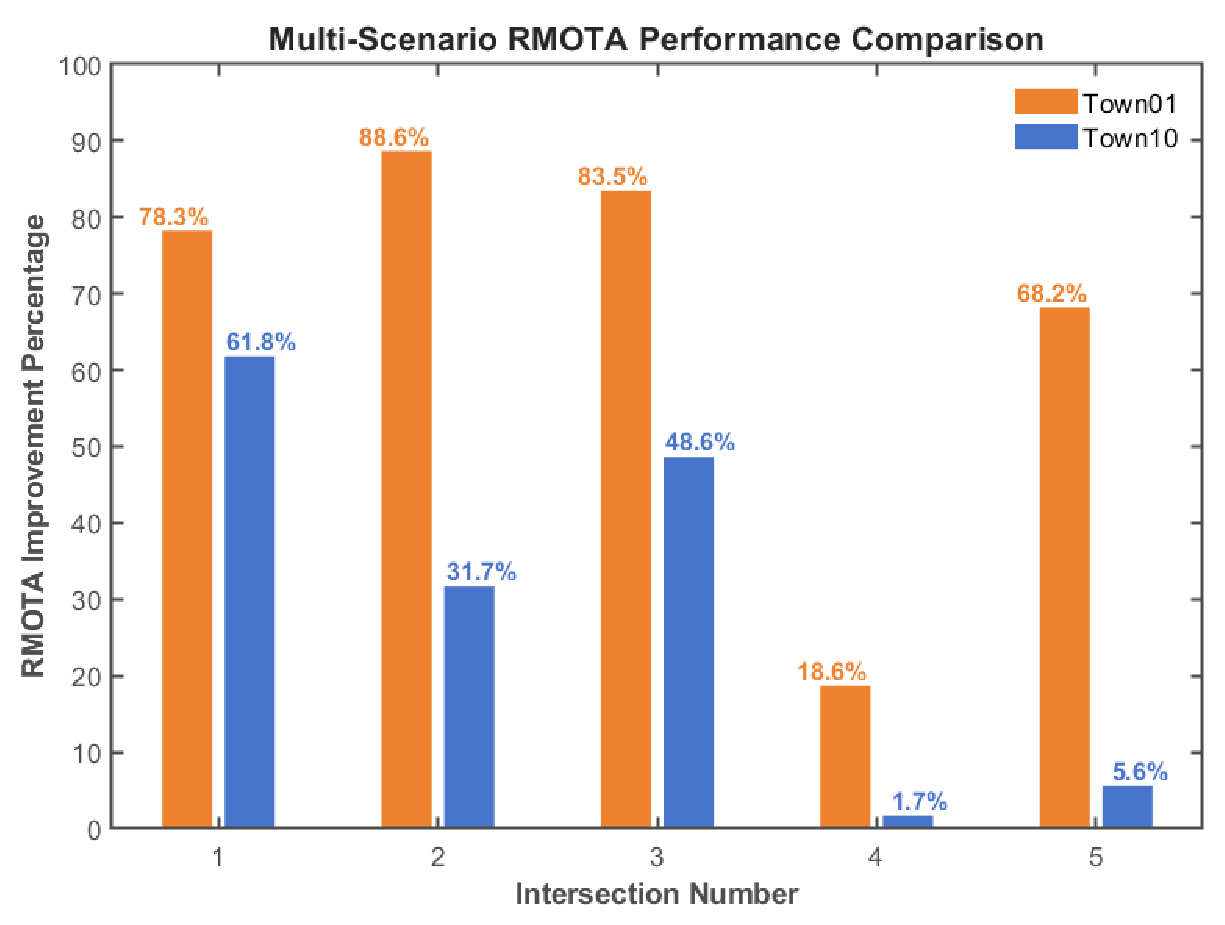
\includegraphics[width=\columnwidth]{picture/picture4.eps}}
	\caption{Comparison of \(RMOTA\) improvement (\%) after hyperparameter optimization on Town01 and Town10. The results demonstrate the effectiveness of the optimization strategies used in different scenarios.} 
	\label{fig:4} 
\end{figure}

\begin{table}[t]
	\centering
	\caption{Optimized Multi-Object Tracking Parameters}
	\label{tab:4}
	\renewcommand\arraystretch{1.2}
	\begin{tabular}{l c ccccc}
		\toprule
		\textbf{Scene} & \textbf{Int.} & \textbf{DP} & \textbf{NTD} & \textbf{CT} & \textbf{DT} & \textbf{DR} \\
		\midrule
		\multirow{5}{*}{Town01} 
		& 1 & 0.8241 & 6.9471e-06 & 0.9592 & 0.4761 & 0.4375 \\
		& 2 & 0.8638 & 2.6997e-06 & 0.9797 & 0.5624 & 0.4379 \\
		& 3 & 0.8457 & 4.2056e-07 & 0.9885 & 0.4010 & 0.5313 \\
		& 4 & 0.7049 & 1.2832e-07 & 0.9860 & 0.5936 & 0.5998 \\
		& 5 & 0.7083 & 4.1939e-06 & 0.9864 & 0.2173 & 0.6836 \\
%		\addlinespace
		\multirow{5}{*}{Town10} 
		& 1 & 0.8993 & 2.5475e-07 & 0.8114 & 0.3347 & 0.5774 \\
		& 2 & 0.8849 & 3.5089e-06 & 0.9711 & 0.5980 & 0.6838 \\
		& 3 & 0.8123 & 1.4860e-07 & 0.9895 & 0.5577 & 0.6986 \\
		& 4 & 0.8594 & 3.3980e-06 & 0.9803 & 0.5654 & 0.5011 \\
		& 5 & 0.8852 & 2.0860e-06 & 0.9817 & 0.5634 & 0.6684 \\
		\bottomrule
	\end{tabular}
\end{table}


\begin{figure}[!t]
	\centerline{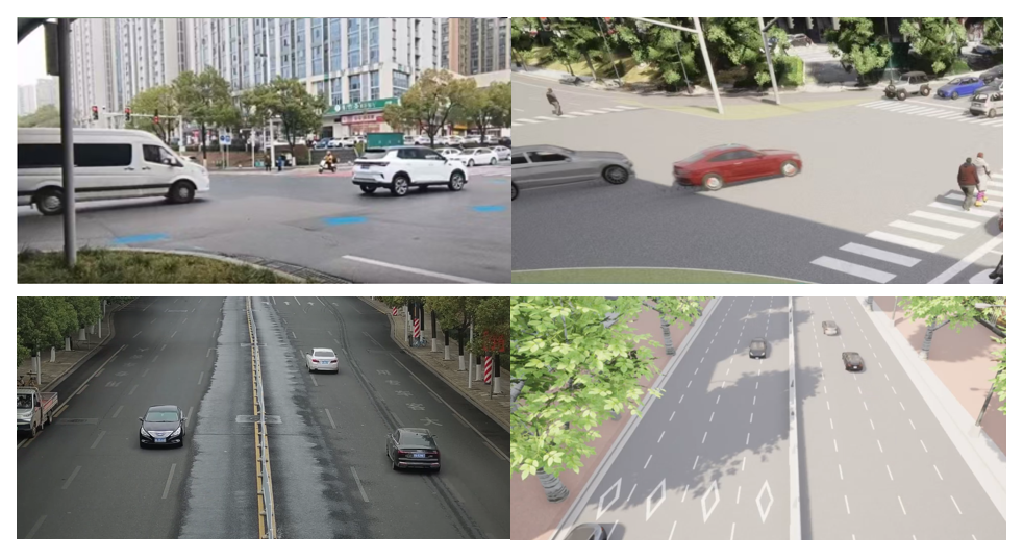
\includegraphics[width=\columnwidth]{picture/picture8.eps}}
	\caption{Our UTDT framework is successfully deployed in two other custom city scenes. Top: Changsha CEC Software Park. Bottom: Hunan University of Technology and Business. (Left) Real scene; (Right) Digital twin.} 
	\label{fig:8} 
\end{figure}
\subsection{Limitations and Future Directions}

\textcolor{red}{As shown in Fig. \ref{fig:8}, although this study successfully reproduced the system in multiple real-world scenarios, several limitations remain.
First, the vehicle images required for cross-intersection trajectory matching are difficult to acquire reliably, affecting appearance-based re-identification feature extraction.
Simultaneously, the limited detection accuracy of the PointPillars model and errors in vehicle image feature matching further propagate these errors to the Siamese twin construction stage.
Furthermore, the current system still relies on offline processing, failing to meet real-time requirements.
In the future, we will improve the system's real-time performance through algorithm acceleration, parallel computing, and online framework migration, and conduct validation in more complex real-world traffic environments to further evaluate its effectiveness and robustness.}

\section{Conclusion}

%With the increasing complexity of urban traffic environments, achieving a unified and consistent digital representation of traffic flow has become crucial for intelligent transportation and autonomous driving. This study presented a unified traffic digital twin (UTDT) framework that integrates multi-sensor perception, trajectory inference, and cross-intersection spatiotemporal association.
%We first introduced the design of the multi-intersection sensing system and data fusion strategy.
%Then, we proposed a re-identification–based trajectory association mechanism and a trajectory reconstruction method to enhance multi-scene continuity.
%Furthermore, we developed several evaluation metrics to assess system performance from single-intersection tracking to digital twin fidelity.
%Finally, the results demonstrate that UTDT provides a feasible foundation for cross-scene traffic reconstruction and verification.
%In future work, we plan to extend the communication and feedback mechanisms between the virtual sensing, planning, and control modules, aiming to gradually bridge the virtual simulation and physical systems to achieve a closed-loop digital twin and real-time optimization.
\textcolor{red}{With the growing complexity of urban traffic, achieving a unified and consistent digital representation has become essential for intelligent transportation and autonomous driving.
This study proposes a unified traffic digital twin (UTDT) framework that integrates multi-sensor perception, trajectory inference, and cross-intersection spatiotemporal association.
We describe the multi-intersection sensing architecture, the ReID-based trajectory association and reconstruction strategy, and the evaluation metrics for both single-intersection tracking and digital twin fidelity.
Experimental results verify that UTDT enables coherent cross-scene traffic reconstruction and system validation. Future work will enhance interaction among sensing, planning, and control modules to progressively realize a closed-loop digital twin capable of real-time optimization.}

\section{Acknowledgements}
The authors gratefully acknowledge the financial support provided by the Natural Science Foundation of Hunan Province (No.2024JJ6190, 2024JK2007-1), the Key project of Xiangjiang Laboratory (25XJ02003), Research on a new generation of brain-like intelligent computing framework based on ultra-large-scale real neural systems (No.24XJJCYJ01001), Scientific research project of Hunan Provincial Department of Education (No.22B0646), the Open Project of Xiangjiang Laboratory (No.23XJ03009), Xiangjiang Laboratory key project subproject (No.22XJ01001-2), the “Digital Intelligence +” interdisciplinary research project of Hunan University Of Technology and Business (No.2023SZJ19).

\bibliographystyle{IEEEtran}
\bibliography{reference}


\begin{IEEEbiography}[{\includegraphics[width=1in,height=1.25in,clip,keepaspectratio]{authors/HaidongWang/HaidongWang.eps}}]{Haidong Wang} received the B.E. degree in Computer Science and Technology from Hunan University Of Technology and Business, Changsha, China, in 2014, the M.Sc. degree in Computer Technology from the University of Chinese Academy of Sciences (UCAS), Beijing, China, in 2017, and Ph.D. degree in Hunan University, Changsha, China. His current research interests include brain-like vision, deep learning and reinforcement learning.
\end{IEEEbiography}

\begin{IEEEbiography}[{\includegraphics[width=1in,height=1.25in,clip,keepaspectratio]{authors/PengfeiXiao/PengfeiXiao.eps}}]{Pengfei Xiao} received the B.E. degree in Computer Science and Technology from Changsha College, China, in 2022, and is now studying in Hunan University Of Technology and Business, Changsha, China, pursuing a professional type master's degree in Computer Technology. His current research interests include brain-like perception, deep learning and autonomous driving.
\end{IEEEbiography}

\begin{IEEEbiography}[{\includegraphics[width=1in,height=1.25in,clip,keepaspectratio]{authors/AoLiu/AoLiu.eps}}]{Ao Liu} received the B.E. degree in Computer Science and Technology from Changsha College, China, in 2023, and is now studying in Hunan University Of Technology and Business, Changsha, China, pursuing a professional type master's degree in Computer Technology. His current research interests include brain-like control and deep learning.
\end{IEEEbiography}

\begin{IEEEbiography}[{\includegraphics[width=1in,height=1.25in,clip,keepaspectratio]{authors/QiaShan/QiaShan.eps}}]{Qia Shan} received the B.E. degree in Network Engineering from Hainan University, Haikou, China, in 2020, and is currently pursuing the M.Sc. degree in Software Engineering at Hunan University Of Technology and Business, Changsha, China. His current research interests include brain-like affective computing and deep learning.
\end{IEEEbiography}
\begin{IEEEbiography}[{\includegraphics[width=1in,height=1.25in,clip,keepaspectratio]{authors/JianhuaZhang/JianhuaZhang.eps}}]{Jianhua Zhang} received the B.E. degree in Software Engineering from Taiyuan University of Technology, TaiYuan, China, in 2022,and M.Sc. degree in Software Engineering from the Hunan University Of Technology and Business, Changsha, China. His current research interests include brain-like vision and deep learning.
\end{IEEEbiography}

\end{document}


